% Options for packages loaded elsewhere
\PassOptionsToPackage{unicode}{hyperref}
\PassOptionsToPackage{hyphens}{url}
\PassOptionsToPackage{dvipsnames,svgnames,x11names}{xcolor}
%
\documentclass[
  letterpaper,
  DIV=11,
  numbers=noendperiod]{scrreport}

\usepackage{amsmath,amssymb}
\usepackage{lmodern}
\usepackage{iftex}
\ifPDFTeX
  \usepackage[T1]{fontenc}
  \usepackage[utf8]{inputenc}
  \usepackage{textcomp} % provide euro and other symbols
\else % if luatex or xetex
  \usepackage{unicode-math}
  \defaultfontfeatures{Scale=MatchLowercase}
  \defaultfontfeatures[\rmfamily]{Ligatures=TeX,Scale=1}
\fi
% Use upquote if available, for straight quotes in verbatim environments
\IfFileExists{upquote.sty}{\usepackage{upquote}}{}
\IfFileExists{microtype.sty}{% use microtype if available
  \usepackage[]{microtype}
  \UseMicrotypeSet[protrusion]{basicmath} % disable protrusion for tt fonts
}{}
\makeatletter
\@ifundefined{KOMAClassName}{% if non-KOMA class
  \IfFileExists{parskip.sty}{%
    \usepackage{parskip}
  }{% else
    \setlength{\parindent}{0pt}
    \setlength{\parskip}{6pt plus 2pt minus 1pt}}
}{% if KOMA class
  \KOMAoptions{parskip=half}}
\makeatother
\usepackage{xcolor}
\setlength{\emergencystretch}{3em} % prevent overfull lines
\setcounter{secnumdepth}{5}
% Make \paragraph and \subparagraph free-standing
\ifx\paragraph\undefined\else
  \let\oldparagraph\paragraph
  \renewcommand{\paragraph}[1]{\oldparagraph{#1}\mbox{}}
\fi
\ifx\subparagraph\undefined\else
  \let\oldsubparagraph\subparagraph
  \renewcommand{\subparagraph}[1]{\oldsubparagraph{#1}\mbox{}}
\fi

\usepackage{color}
\usepackage{fancyvrb}
\newcommand{\VerbBar}{|}
\newcommand{\VERB}{\Verb[commandchars=\\\{\}]}
\DefineVerbatimEnvironment{Highlighting}{Verbatim}{commandchars=\\\{\}}
% Add ',fontsize=\small' for more characters per line
\usepackage{framed}
\definecolor{shadecolor}{RGB}{241,243,245}
\newenvironment{Shaded}{\begin{snugshade}}{\end{snugshade}}
\newcommand{\AlertTok}[1]{\textcolor[rgb]{0.68,0.00,0.00}{#1}}
\newcommand{\AnnotationTok}[1]{\textcolor[rgb]{0.37,0.37,0.37}{#1}}
\newcommand{\AttributeTok}[1]{\textcolor[rgb]{0.40,0.45,0.13}{#1}}
\newcommand{\BaseNTok}[1]{\textcolor[rgb]{0.68,0.00,0.00}{#1}}
\newcommand{\BuiltInTok}[1]{\textcolor[rgb]{0.00,0.23,0.31}{#1}}
\newcommand{\CharTok}[1]{\textcolor[rgb]{0.13,0.47,0.30}{#1}}
\newcommand{\CommentTok}[1]{\textcolor[rgb]{0.37,0.37,0.37}{#1}}
\newcommand{\CommentVarTok}[1]{\textcolor[rgb]{0.37,0.37,0.37}{\textit{#1}}}
\newcommand{\ConstantTok}[1]{\textcolor[rgb]{0.56,0.35,0.01}{#1}}
\newcommand{\ControlFlowTok}[1]{\textcolor[rgb]{0.00,0.23,0.31}{#1}}
\newcommand{\DataTypeTok}[1]{\textcolor[rgb]{0.68,0.00,0.00}{#1}}
\newcommand{\DecValTok}[1]{\textcolor[rgb]{0.68,0.00,0.00}{#1}}
\newcommand{\DocumentationTok}[1]{\textcolor[rgb]{0.37,0.37,0.37}{\textit{#1}}}
\newcommand{\ErrorTok}[1]{\textcolor[rgb]{0.68,0.00,0.00}{#1}}
\newcommand{\ExtensionTok}[1]{\textcolor[rgb]{0.00,0.23,0.31}{#1}}
\newcommand{\FloatTok}[1]{\textcolor[rgb]{0.68,0.00,0.00}{#1}}
\newcommand{\FunctionTok}[1]{\textcolor[rgb]{0.28,0.35,0.67}{#1}}
\newcommand{\ImportTok}[1]{\textcolor[rgb]{0.00,0.46,0.62}{#1}}
\newcommand{\InformationTok}[1]{\textcolor[rgb]{0.37,0.37,0.37}{#1}}
\newcommand{\KeywordTok}[1]{\textcolor[rgb]{0.00,0.23,0.31}{#1}}
\newcommand{\NormalTok}[1]{\textcolor[rgb]{0.00,0.23,0.31}{#1}}
\newcommand{\OperatorTok}[1]{\textcolor[rgb]{0.37,0.37,0.37}{#1}}
\newcommand{\OtherTok}[1]{\textcolor[rgb]{0.00,0.23,0.31}{#1}}
\newcommand{\PreprocessorTok}[1]{\textcolor[rgb]{0.68,0.00,0.00}{#1}}
\newcommand{\RegionMarkerTok}[1]{\textcolor[rgb]{0.00,0.23,0.31}{#1}}
\newcommand{\SpecialCharTok}[1]{\textcolor[rgb]{0.37,0.37,0.37}{#1}}
\newcommand{\SpecialStringTok}[1]{\textcolor[rgb]{0.13,0.47,0.30}{#1}}
\newcommand{\StringTok}[1]{\textcolor[rgb]{0.13,0.47,0.30}{#1}}
\newcommand{\VariableTok}[1]{\textcolor[rgb]{0.07,0.07,0.07}{#1}}
\newcommand{\VerbatimStringTok}[1]{\textcolor[rgb]{0.13,0.47,0.30}{#1}}
\newcommand{\WarningTok}[1]{\textcolor[rgb]{0.37,0.37,0.37}{\textit{#1}}}

\providecommand{\tightlist}{%
  \setlength{\itemsep}{0pt}\setlength{\parskip}{0pt}}\usepackage{longtable,booktabs,array}
\usepackage{calc} % for calculating minipage widths
% Correct order of tables after \paragraph or \subparagraph
\usepackage{etoolbox}
\makeatletter
\patchcmd\longtable{\par}{\if@noskipsec\mbox{}\fi\par}{}{}
\makeatother
% Allow footnotes in longtable head/foot
\IfFileExists{footnotehyper.sty}{\usepackage{footnotehyper}}{\usepackage{footnote}}
\makesavenoteenv{longtable}
\usepackage{graphicx}
\makeatletter
\def\maxwidth{\ifdim\Gin@nat@width>\linewidth\linewidth\else\Gin@nat@width\fi}
\def\maxheight{\ifdim\Gin@nat@height>\textheight\textheight\else\Gin@nat@height\fi}
\makeatother
% Scale images if necessary, so that they will not overflow the page
% margins by default, and it is still possible to overwrite the defaults
% using explicit options in \includegraphics[width, height, ...]{}
\setkeys{Gin}{width=\maxwidth,height=\maxheight,keepaspectratio}
% Set default figure placement to htbp
\makeatletter
\def\fps@figure{htbp}
\makeatother
\newlength{\cslhangindent}
\setlength{\cslhangindent}{1.5em}
\newlength{\csllabelwidth}
\setlength{\csllabelwidth}{3em}
\newlength{\cslentryspacingunit} % times entry-spacing
\setlength{\cslentryspacingunit}{\parskip}
\newenvironment{CSLReferences}[2] % #1 hanging-ident, #2 entry spacing
 {% don't indent paragraphs
  \setlength{\parindent}{0pt}
  % turn on hanging indent if param 1 is 1
  \ifodd #1
  \let\oldpar\par
  \def\par{\hangindent=\cslhangindent\oldpar}
  \fi
  % set entry spacing
  \setlength{\parskip}{#2\cslentryspacingunit}
 }%
 {}
\usepackage{calc}
\newcommand{\CSLBlock}[1]{#1\hfill\break}
\newcommand{\CSLLeftMargin}[1]{\parbox[t]{\csllabelwidth}{#1}}
\newcommand{\CSLRightInline}[1]{\parbox[t]{\linewidth - \csllabelwidth}{#1}\break}
\newcommand{\CSLIndent}[1]{\hspace{\cslhangindent}#1}

\usepackage{booktabs}
\usepackage{longtable}
\usepackage{array}
\usepackage{multirow}
\usepackage{wrapfig}
\usepackage{float}
\usepackage{colortbl}
\usepackage{pdflscape}
\usepackage{tabu}
\usepackage{threeparttable}
\usepackage{threeparttablex}
\usepackage[normalem]{ulem}
\usepackage{makecell}
\usepackage{xcolor}
\KOMAoption{captions}{tableheading}
\makeatletter
\makeatother
\makeatletter
\@ifpackageloaded{bookmark}{}{\usepackage{bookmark}}
\makeatother
\makeatletter
\@ifpackageloaded{caption}{}{\usepackage{caption}}
\AtBeginDocument{%
\ifdefined\contentsname
  \renewcommand*\contentsname{Table of contents}
\else
  \newcommand\contentsname{Table of contents}
\fi
\ifdefined\listfigurename
  \renewcommand*\listfigurename{List of Figures}
\else
  \newcommand\listfigurename{List of Figures}
\fi
\ifdefined\listtablename
  \renewcommand*\listtablename{List of Tables}
\else
  \newcommand\listtablename{List of Tables}
\fi
\ifdefined\figurename
  \renewcommand*\figurename{Figure}
\else
  \newcommand\figurename{Figure}
\fi
\ifdefined\tablename
  \renewcommand*\tablename{Table}
\else
  \newcommand\tablename{Table}
\fi
}
\@ifpackageloaded{float}{}{\usepackage{float}}
\floatstyle{ruled}
\@ifundefined{c@chapter}{\newfloat{codelisting}{h}{lop}}{\newfloat{codelisting}{h}{lop}[chapter]}
\floatname{codelisting}{Listing}
\newcommand*\listoflistings{\listof{codelisting}{List of Listings}}
\makeatother
\makeatletter
\@ifpackageloaded{caption}{}{\usepackage{caption}}
\@ifpackageloaded{subcaption}{}{\usepackage{subcaption}}
\makeatother
\makeatletter
\@ifpackageloaded{tcolorbox}{}{\usepackage[many]{tcolorbox}}
\makeatother
\makeatletter
\@ifundefined{shadecolor}{\definecolor{shadecolor}{rgb}{.97, .97, .97}}
\makeatother
\makeatletter
\makeatother
\ifLuaTeX
  \usepackage{selnolig}  % disable illegal ligatures
\fi
\IfFileExists{bookmark.sty}{\usepackage{bookmark}}{\usepackage{hyperref}}
\IfFileExists{xurl.sty}{\usepackage{xurl}}{} % add URL line breaks if available
\urlstyle{same} % disable monospaced font for URLs
\hypersetup{
  pdftitle={Defining Data Science},
  pdfauthor={Xinrui WANG and Tsai-Chun TSOU},
  colorlinks=true,
  linkcolor={blue},
  filecolor={Maroon},
  citecolor={Blue},
  urlcolor={Blue},
  pdfcreator={LaTeX via pandoc}}

\title{Defining Data Science}
\usepackage{etoolbox}
\makeatletter
\providecommand{\subtitle}[1]{% add subtitle to \maketitle
  \apptocmd{\@title}{\par {\large #1 \par}}{}{}
}
\makeatother
\subtitle{A Case Study in Australia}
\author{Xinrui WANG and Tsai-Chun TSOU}
\date{`28 October 2022}

\begin{document}
\maketitle
\ifdefined\Shaded\renewenvironment{Shaded}{\begin{tcolorbox}[enhanced, borderline west={3pt}{0pt}{shadecolor}, frame hidden, boxrule=0pt, interior hidden, breakable, sharp corners]}{\end{tcolorbox}}\fi

\renewcommand*\contentsname{Table of contents}
{
\hypersetup{linkcolor=}
\setcounter{tocdepth}{2}
\tableofcontents
}
\bookmarksetup{startatroot}

\hypertarget{preface}{%
\chapter*{Preface}\label{preface}}
\addcontentsline{toc}{chapter}{Preface}

What is Data Science? What do you learn in Data Science? What kind of
jobs do Data Scientists do? These are the type of questions we've
encountered during social occasions and despite spending almost two
years studying Business Analytics, we still struggle to give a definite
answer. Data Science, Business Analysis, and Data Analysis are new
degrees that are created only in recent years thanks to the advance in
technology and increasing demand for talent to work with data. The
sudden rise of these degrees gave authorities little time to regulate
them. Even the Australian and New Zealand Standard Classification of
Occupations (ANZSCO), the Australian Bureau of Statistics (ABS) and the
Department of Home Affair are slow to catch up with their
\href{https://www.hannantew.com.au/blogs/australian-visas/employer-sponsored/tss/the-classification-challenge-in-immigration-what-is-a-data-scientist-as-defined-in-anzsco/}{description}
of this occupation.

After four months of gathering data, conducting analysis, and running
models, we have attempted to define Data Science in Australia. Special
thanks to Professor Di Cook and Professor Rob Hyndman for their support.
A huge thank you to Dr.~Emi Tanaka for the opportunity to work on such a
special project and for her guidance throughout the semester\footnote{This
  report is written jointly by Tsai-Chun Tsou and Xinrui Wang as part of
  the ETC5543 research project supervised by Dr.~Emi Tanaka.}.

\bookmarksetup{startatroot}

\hypertarget{abstract}{%
\chapter{Abstract}\label{abstract}}

With the increase in demand for data scientist and the rising popularity
of the degrees, how does one define Data Science in Australia. The
Australian Mathematical Sciences Institute (AMSI) and the Statistical
Society of Australia (SSA) are conducting a review of Australian Data
Science Degrees with
\href{https://amsi.org.au/amsi-ssa-data-science-review/}{surveys} and
focus groups. The survey method is prone to biases due to the subjective
nature. Our research attempts to tackle similar topic but with a more
objective approach by collecting data directly from public resources. We
collected Data Science related unit information from Group of Eight
Universities and
\href{(https://www.kaggle.com/code/nomilk/exploring-2-years-of-data-scientist-job-listings/data)}{Data
Scientist Job Listings} from kaggle. We used the data to decompose the
core disciplines involved in the degree as well the type of skill sets
that may be required. To expand on the initial exploratory data
analysis, we also build Latent Dirichlet Allocation models to construct
our own text corpus.

From the exploratory data analysis, we observe a lack of homogeneity
within the Universities' analysis. The inconsistent data metrics made it
difficult to draw direct comparison between the employer data and
university data. Nonetheless we were able to conclude that computational
disciplines are more prominent on both sides.

\bookmarksetup{startatroot}

\hypertarget{introduction}{%
\chapter{Introduction}\label{introduction}}

Data Science has ranked as one of the most in-demand jobs in Australia
in recent consecutive years. As demands steadily grows, students are
also increasingly interested in Data Science degrees, yet recruiters
still seem to struggle to fill up data science positions. This leads to
our main question: what is Data Science? Is there a shared structure or
skill set of Data Science courses offered at Australian universities?
Are students and employers' perception of data science similar? To
answer these questions, we looked a data from both University and
Employer perspectives.

There is no readily available data from Australian universities, so we
had to build our own data set through web scraping. The initial target
was to collect data from all universities in Australia including both
undergraduate and postgraduate courses, however, due to time constrain,
the data collected for this project only contains Master of Data Science
courses from the Group of Eight (Go8) universities. The employer data
was retrieved from
\href{(https://www.kaggle.com/code/nomilk/exploring-2-years-of-data-scientist-job-listings/data)}{Data
Scientist Job Listings} on kaggle.

By exploring the current situation and potentially a definition of Data
Science in Australia from both university and employer perspectives, the
findings would help students and recruiters have a clearer picture of
what to expect, as well as raising attentions and awareness to potential
gaps between employer demands and university offerings.

\part{Data Collection}

\hypertarget{university-data}{%
\chapter{University Data}\label{university-data}}

\hypertarget{web-scraping}{%
\section{Web Scraping}\label{web-scraping}}

In order to explore the Data Science degrees around Australia
Universities, we compiled a list of universities in Australia and the
Data Science or related degrees they offered, then web scraped required
information from each university's website using R. In total, we
collected 298 units from eight postgraduate courses in Data Science
across all Group of Eight (Go8) universities.

To start off the project, Professor Tanaka provided sample code for data
scraping using Monash Handbook as an example. Libraries \texttt{rvest}
and \texttt{rSelenium} are two of the main tools. Initially, we studied
her code and then tried to replicate her code to be applied to other
university's websites.

The flow of the data scraping is as follow (example code from
\texttt{uom-master-datasci.qmd}):

\begin{enumerate}
\def\labelenumi{\arabic{enumi}.}
\tightlist
\item
  Identify the main page (url) where the degree information is
  contained, which usually is the most updated version of the handbook.
\end{enumerate}

\begin{Shaded}
\begin{Highlighting}[]
\NormalTok{remDr}\SpecialCharTok{$}\FunctionTok{navigate}\NormalTok{(}\StringTok{"https://handbook.unimelb.edu.au/2022/courses/mc{-}datasc/course{-}structure"}\NormalTok{)}
\NormalTok{sub\_list }\OtherTok{\textless{}{-}} \FunctionTok{read\_html}\NormalTok{(remDr}\SpecialCharTok{$}\FunctionTok{getPageSource}\NormalTok{()[[}\DecValTok{1}\NormalTok{]])}
\end{Highlighting}
\end{Shaded}

\begin{enumerate}
\def\labelenumi{\arabic{enumi}.}
\setcounter{enumi}{1}
\tightlist
\item
  Use functions from \texttt{rvest} to retrieve all the course unit code
  (or course unit url). Retrieve the degree code and formal degree name
  and save it for later.
\end{enumerate}

\begin{Shaded}
\begin{Highlighting}[]
\NormalTok{curriculum }\OtherTok{\textless{}{-}}\NormalTok{ sub\_list }\SpecialCharTok{\%\textgreater{}\%} 
      \FunctionTok{html\_element}\NormalTok{(}\StringTok{"\#top"}\NormalTok{) }\SpecialCharTok{\%\textgreater{}\%} 
      \FunctionTok{html\_element}\NormalTok{(}\StringTok{".mobile{-}wrap"}\NormalTok{) }\SpecialCharTok{\%\textgreater{}\%} 
      \FunctionTok{html\_elements}\NormalTok{(}\StringTok{"table"}\NormalTok{) }\SpecialCharTok{\%\textgreater{}\%} 
      \FunctionTok{html\_elements}\NormalTok{(}\StringTok{"a"}\NormalTok{) }\SpecialCharTok{\%\textgreater{}\%} 
      \FunctionTok{html\_attr}\NormalTok{(}\StringTok{"href"}\NormalTok{)}
\end{Highlighting}
\end{Shaded}

\begin{enumerate}
\def\labelenumi{\arabic{enumi}.}
\setcounter{enumi}{2}
\item
  Use \texttt{rSelenium} functions and course unit information, to
  direct R to the unit information page.
\item
  Retrieve the following information from the page using rvest
  functions:

  \begin{itemize}
  \tightlist
  \item
    Unit Name
  \item
    Unit Code
  \item
    Unit Overview
  \item
    Unit Learning Outcome
  \item
    Unit Prohibition/ Pre-requisite/ Co-requisite
  \end{itemize}
\item
  Repeat step 3 \& 4 with loop function.
\end{enumerate}

\begin{Shaded}
\begin{Highlighting}[]
\ControlFlowTok{for}\NormalTok{(unit }\ControlFlowTok{in}\NormalTok{ curriculum) \{}
\NormalTok{      remDr}\SpecialCharTok{$}\FunctionTok{navigate}\NormalTok{(}\FunctionTok{glue}\NormalTok{(}\StringTok{"\{baseurl\}\{unit\}"}\NormalTok{))}
      \FunctionTok{wait\_time}\NormalTok{()}
\NormalTok{      unit\_html }\OtherTok{\textless{}{-}} \FunctionTok{read\_html}\NormalTok{(remDr}\SpecialCharTok{$}\FunctionTok{getPageSource}\NormalTok{()[[}\DecValTok{1}\NormalTok{]])}
      
      \CommentTok{\# unit name}
\NormalTok{      subject\_text }\OtherTok{\textless{}{-}}\NormalTok{ unit\_html }\SpecialCharTok{\%\textgreater{}\%} 
        \FunctionTok{html\_element}\NormalTok{(}\StringTok{"h1"}\NormalTok{) }\SpecialCharTok{\%\textgreater{}\%} 
        \FunctionTok{html\_text}\NormalTok{()}
\NormalTok{        ...}
\end{Highlighting}
\end{Shaded}

\begin{enumerate}
\def\labelenumi{\arabic{enumi}.}
\setcounter{enumi}{5}
\tightlist
\item
  Compile all the retrieved data from the University into a dataframe
  and export it as csv file.
\end{enumerate}

\begin{Shaded}
\begin{Highlighting}[]
\NormalTok{data }\OtherTok{\textless{}{-}}\NormalTok{ data }\SpecialCharTok{\%\textgreater{}\%} 
        \FunctionTok{bind\_rows}\NormalTok{(}\FunctionTok{tibble}\NormalTok{(}\SpecialCharTok{!!!}\FunctionTok{c}\NormalTok{(}\FunctionTok{list}\NormalTok{(}\AttributeTok{Course =}\NormalTok{ title, }
                                   \CommentTok{\#Course\_code = "MC{-}DATASC", }
                                   \AttributeTok{Course\_overview =} \FunctionTok{paste0}\NormalTok{(coverview, }\AttributeTok{collapse =} \StringTok{" "}\NormalTok{),}
                                   \CommentTok{\#Unit\_code = cunit,}
                                   \AttributeTok{Unit =}\NormalTok{ subject\_text,}
                                   \AttributeTok{Overview =}\NormalTok{ overview,}
                                   \AttributeTok{Prerequisite =} \FunctionTok{paste0}\NormalTok{(pre, }\AttributeTok{collapse =} \StringTok{", "}\NormalTok{),}
                                   \AttributeTok{Corequisite =}\NormalTok{ co,}
                                   \AttributeTok{Prohibition =} \FunctionTok{paste0}\NormalTok{(pro, }\AttributeTok{collapse =} \StringTok{", "}\NormalTok{),}
                                   \AttributeTok{Outcomes =}\NormalTok{lo}
\NormalTok{                                   ))))}
\end{Highlighting}
\end{Shaded}

Despite the process being similar for each University, we soon realize
the process was going to be more challenging than expected.

\hypertarget{inconsistent-information}{%
\section{Inconsistent Information}\label{inconsistent-information}}

Monash University's student handbook on Degrees and Courses is a
spectacular website for data scraping. Its html code is clearly labeled
and anything you need to know about the degree or course can be found on
the website. The same cannot be said about other universities.

The course descriptions on the handbook and universities' website page
are usually structured in a different manner, since the majority of the
data is collected from universities' handbooks, course descriptions are
also extracted from handbooks for consistency purposes.

In addition, the required unit information listed above is not all
available at the targeted universities. The handbook from University of
New South Wales contains extremely limited information: unit overview is
brief, unit requisites are only available for a few units, and unit
outcome is not provided at all.

\hypertarget{difficult-to-manage-websites}{%
\section{Difficult to Manage
Websites}\label{difficult-to-manage-websites}}

Each university website is unique. Sometimes the information is not
straightforward. An example of this is University of Adelaide. The main
website for the degree does contain the list of units that go into the
degree.

However, instead of having just one page with all the unit information,
the link takes you to a page with different unit information depending
on when the unit is offered and on what campus.

Tina tried bypassing the pages by directly looking at the url of the
final unit information page I want to be on. Unfortunately, the url is
not designed or structured in a way which she was able to predict the
url based on the current unit code. With that said, her only option was
to code the function to jump from pages to pages before landing on the
right unit information page.

It is also often found that the unit overview and learning outcomes for
each unit within the same university could vary slightly in format. For
example, unit overview may appears before or after campus location at
University of Western Australia, empty spaces could be found after
section title at the University of Melbourne, which would break the
chain of extracting corresponding information.

\hypertarget{collected-data}{%
\section{Collected Data}\label{collected-data}}

The collected data contains \textbf{298 units} from 8 universities, and
\textbf{8 variables} including School, Course, Course\_code, Unit,
Unit\_code, Outcomes, Overview and Description. The full data set is
made available below for exploration.


\includegraphics{./03_1-webscraping_files/figure-pdf/unnamed-chunk-1-1.pdf}

\hypertarget{employer-data}{%
\chapter{Employer Data}\label{employer-data}}

For employer's perception of Data Science, we decided to look at the job
postings for Data Science relevant positions. We would have scraped
career websites given more time. However, due to the circumstances, we
found readily available data from
\href{https://www.kaggle.com/code/nomilk/exploring-2-years-of-data-scientist-job-listings/data}{Exploring
2 years' of Data Scientist Job Listings}.

\hypertarget{data-science-job-postings}{%
\section{Data Science Job Postings}\label{data-science-job-postings}}

The data was scraped from Seek.com by Steve Condylios. The collected
data contains \textbf{2,857} job posts and \textbf{52 variables}.

Exploratory data analysis was conducted exploring the salary and
breakdown of Go8 emloyers. However they did not yield interesting
results and thus put aside. For the purpose of this report, only 29
variables were looked at, including jobId, jobTitle, jobClassification,
mobileAdTemplate, 25 programming languages. Of all the job posts, 535
are for senior or managerial positions, 25 for graduate positions, and
the rest not specified in the job title.

Condylios also included Data Analyst job posting in the data set. 92
jobs are for Data Analyst and 82 jobs are labeled Data Analyst/Data
Scientist. This is another interesting topic for comparison between Data
Analyst and Data Scientist but for the scope of the project, we do not
delve deeper into the data collection decisions.

The a fraction of the data set is made available below for exploration.

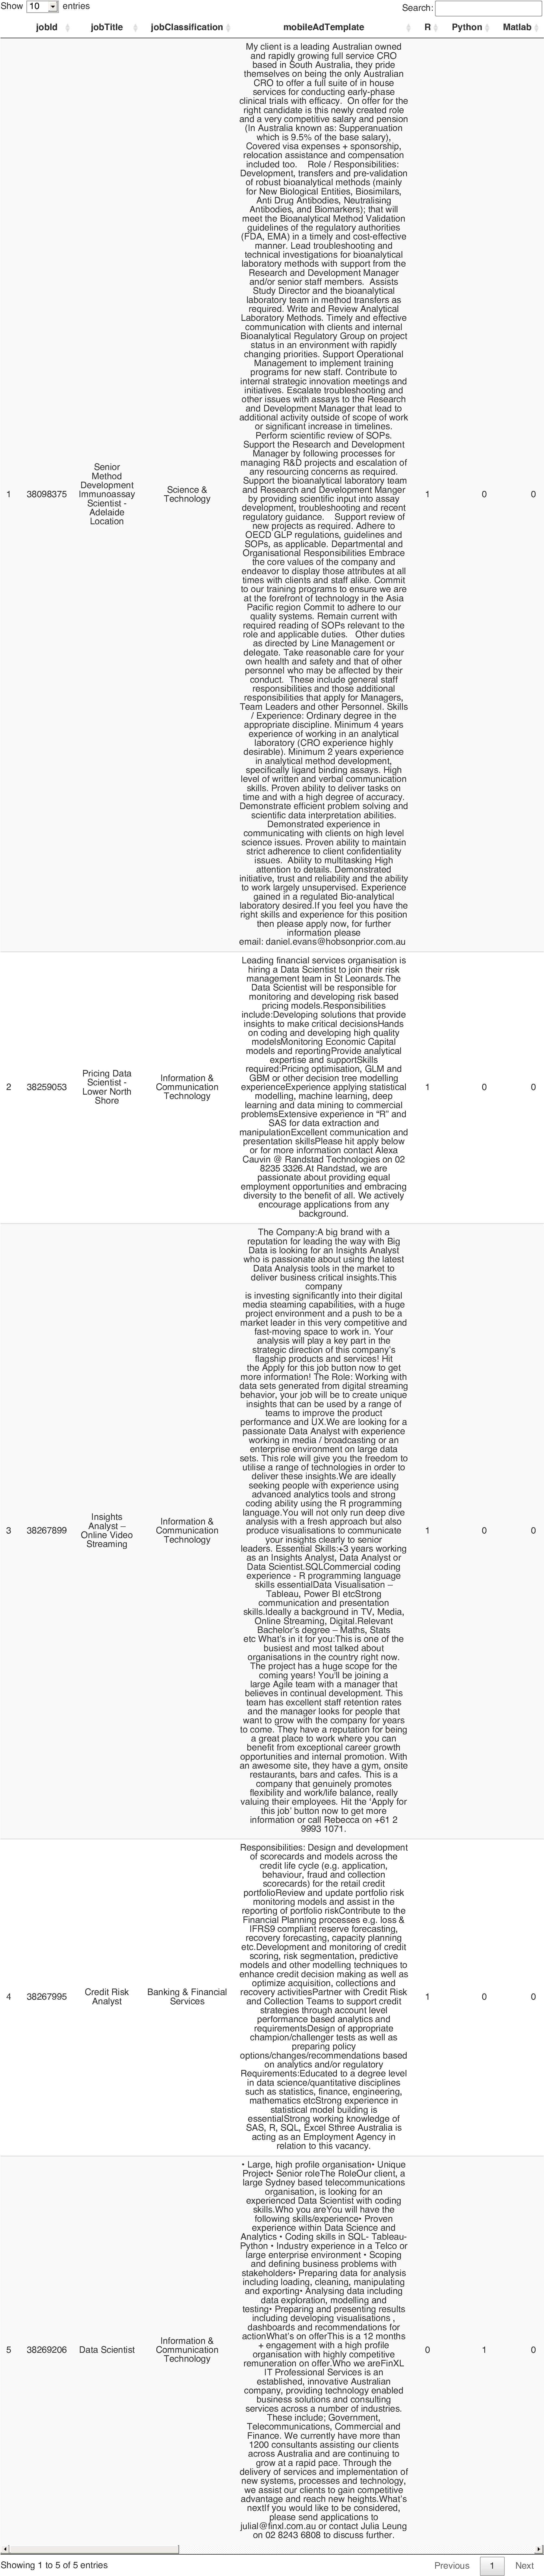
\includegraphics{./03_2-kaggle_files/figure-pdf/employerdf-1.pdf}

\part{Text Analysis}

To find out what is data science from universities' and employers'
perspectives, whether there is a shared structure or common skill set of
Master of Data Science degrees offered at Go8, what employers expect
from a data scientist in the workplace, an exploratory data analysis, in
particular text analysis has been conducted.

For universities, the main purpose is to identify shared skills or
concepts offered by Master of Data Science degrees through exploring
faculty of the units, detailed teaching contents etc. Whereas for
employer data, the focus is to extract information regarding skills and
programming languages in demand.

\hypertarget{unit-text-analysis}{%
\chapter{Unit Text Analysis}\label{unit-text-analysis}}

\hypertarget{sec-unit-code}{%
\section{Unit Code Analysis}\label{sec-unit-code}}

To explore the teaching contents of Master of Data Science at Go8, an
analysis based on faculty of units offered is conducted to see what
components are included in this degree.

Unfortunately faculty information is not directly available on the unit
handbooks, in this case, unit code is taken as a surrogate
identification. As shown in the sample data below, unit code is a
combination of letters and numbers, the first few characters such as
FIT, MAT, usually represents the faculty this unit belongs to, we could
then make relatively educated assumptions on the content of the unit.

\begin{table}
\centering
\begin{tabular}{l|l|l|l}
\hline
School & Course & Unit & Unit\_code\\
\hline
monash & Master of Data Science & FIT9132 - Introduction to databases & FIT9132\\
\hline
monash & Master of Data Science & FIT9136 - Algorithms and programming foundations in Python & FIT9136\\
\hline
monash & Master of Data Science & FIT9137 - Introduction to computer architecture and networks & FIT9137\\
\hline
monash & Master of Data Science & MAT9004 - Mathematical foundations for data science and AI & MAT9004\\
\hline
monash & Master of Data Science & FIT5125 - IT research methods & FIT5125\\
\hline
monash & Master of Data Science & FIT5145 - Introduction to data science & FIT5145\\
\hline
monash & Master of Data Science & FIT5147 - Data exploration and visualisation & FIT5147\\
\hline
monash & Master of Data Science & FIT5196 - Data wrangling & FIT5196\\
\hline
monash & Master of Data Science & FIT5197 - Statistical data modelling & FIT5197\\
\hline
monash & Master of Data Science & FIT5149 - Applied data analysis & FIT5149\\
\hline
monash & Master of Data Science & FIT5201 - Machine learning & FIT5201\\
\hline
monash & Master of Data Science & FIT5202 - Data processing for big data & FIT5202\\
\hline
monash & Master of Data Science & FIT5205 - Data in society & FIT5205\\
\hline
monash & Master of Data Science & FIT5212 - Data analysis for semi-structured data & FIT5212\\
\hline
monash & Master of Data Science & FIT5230 - Malicious AI & FIT5230\\
\hline
monash & Master of Data Science & BMS5021 - Introduction to Bioinformatics & BMS5021\\
\hline
monash & Master of Data Science & BMS5022 - Advanced bioinformatics: efficient genome, transcriptome and proteome analysis & BMS5022\\
\hline
monash & Master of Data Science & FIT5126 - Masters thesis part 1 & FIT5126\\
\hline
monash & Master of Data Science & FIT5127 - Masters thesis part 2 & FIT5127\\
\hline
monash & Master of Data Science & FIT5228 - Masters thesis part 3 & FIT5228\\
\hline
monash & Master of Data Science & FIT5229 - Masters thesis final & FIT5229\\
\hline
monash & Master of Data Science & FIT5120 - Industry experience studio project & FIT5120\\
\hline
monash & Master of Data Science & FIT5122 - Professional practice & FIT5122\\
\hline
unimelb & Master of Data Science & Methods of Mathematical Statistics & MAST90105\\
\hline
unimelb & Master of Data Science & A First Course In Statistical Learning & MAST90104\\
\hline
unimelb & Master of Data Science & Programming and Software Development & COMP90041\\
\hline
unimelb & Master of Data Science & Algorithms and Complexity & COMP90038\\
\hline
unimelb & Master of Data Science & Elements of Data Processing & COMP20008\\
\hline
unimelb & Master of Data Science & Database Systems \& Information Modelling & INFO90002\\
\hline
unimelb & Master of Data Science & Statistical Modelling for Data Science & MAST90139\\
\hline
unimelb & Master of Data Science & Multivariate Statistics for Data Science & MAST90138\\
\hline
unimelb & Master of Data Science & Computational Statistics \& Data Science & MAST90083\\
\hline
unimelb & Master of Data Science & Cluster and Cloud Computing & COMP90024\\
\hline
unimelb & Master of Data Science & Advanced Database Systems & COMP90050\\
\hline
unimelb & Master of Data Science & Statistical Machine Learning & COMP90051\\
\hline
unimelb & Master of Data Science & Data Science Project Pt1 & MAST90106\\
\hline
unimelb & Master of Data Science & Data Science Project Pt2 & MAST90107\\
\hline
unimelb & Master of Data Science & Data Science Research Project Pt1 & MAST90108\\
\hline
unimelb & Master of Data Science & Data Science Research Project Pt2 & MAST90109\\
\hline
unimelb & Master of Data Science & Foundations of Spatial Information & GEOM90008\\
\hline
unimelb & Master of Data Science & Spatial Databases & GEOM90018\\
\hline
unimelb & Master of Data Science & Spatial Analysis & GEOM90006\\
\hline
unimelb & Master of Data Science & Information Visualisation & GEOM90007\\
\hline
unimelb & Master of Data Science & Analysis of High-Dimensional Data & MAST90110\\
\hline
unimelb & Master of Data Science & Advanced Statistical Modelling & MAST90111\\
\hline
unimelb & Master of Data Science & Mathematics of Risk & MAST90051\\
\hline
unimelb & Master of Data Science & Optimisation for Industry & MAST90014\\
\hline
unimelb & Master of Data Science & Practice of Statistics \& Data Science & MAST90027\\
\hline
unimelb & Master of Data Science & Stochastic Calculus with Applications & MAST90059\\
\hline
unimelb & Master of Data Science & Advanced Probability & MAST90081\\
\hline
unimelb & Master of Data Science & Random Processes & MAST90019\\
\hline
unimelb & Master of Data Science & Bayesian Statistical Learning & MAST90125\\
\hline
unimelb & Master of Data Science & Mathematical Statistics & MAST90082\\
\hline
unimelb & Master of Data Science & AI Planning for Autonomy & COMP90054\\
\hline
unimelb & Master of Data Science & Advanced Theoretical Computer Science & COMP90057\\
\hline
unimelb & Master of Data Science & Algorithms for Bioinformatics & COMP90014\\
\hline
unimelb & Master of Data Science & Computational Genomics & COMP90016\\
\hline
unimelb & Master of Data Science & Constraint Programming & COMP90046\\
\hline
unimelb & Master of Data Science & Cryptography and Security & COMP90043\\
\hline
unimelb & Master of Data Science & Declarative Programming & COMP90048\\
\hline
unimelb & Master of Data Science & Distributed Algorithms & COMP90020\\
\hline
unimelb & Master of Data Science & Distributed Systems & COMP90015\\
\hline
unimelb & Master of Data Science & Internet Technologies & COMP90007\\
\hline
unimelb & Master of Data Science & Mobile Computing Systems Programming & COMP90018\\
\hline
unimelb & Master of Data Science & Parallel and Multicore Computing & COMP90025\\
\hline
unimelb & Master of Data Science & Programming Language Implementation & COMP90045\\
\hline
unimelb & Master of Data Science & Natural Language Processing & COMP90042\\
\hline
unimelb & Master of Data Science & Stream Computing and Applications & COMP90056\\
\hline
unimelb & Master of Data Science & Knowledge Management Systems & ISYS90035\\
\hline
unimelb & Master of Data Science & Security Analytics & COMP90073\\
\hline
unimelb & Master of Data Science & Computer Vision & COMP90086\\
\hline
unimelb & Master of Data Science & The Ethics of Artificial Intelligence & COMP90087\\
\hline
unimelb & Master of Data Science & Science in Schools & EDUC90839\\
\hline
unimelb & Master of Data Science & Science and Technology Internship & SCIE90017\\
\hline
unimelb & Master of Data Science & Communicating Science at Work & SCIE90034\\
\hline
usyd & Master of Data Science & Visual Analytics & COMP5048\\
\hline
usyd & Master of Data Science & Principles of Data Science & COMP5310\\
\hline
usyd & Master of Data Science & Machine Learning and Data Mining & COMP5318\\
\hline
usyd & Master of Data Science & Computational Statistical Methods & STAT5003\\
\hline
usyd & Master of Data Science & Data Science Capstone Project & DATA5703\\
\hline
usyd & Master of Data Science & Data Science Capstone A & DATA5707\\
\hline
usyd & Master of Data Science & Data Science Capstone B & DATA5708\\
\hline
usyd & Master of Data Science & Data Science Capstone Project - Individual & DATA5709\\
\hline
usyd & Master of Data Science & Natural Language Processing & COMP5046\\
\hline
usyd & Master of Data Science & Advanced Machine Learning & COMP5328\\
\hline
usyd & Master of Data Science & Deep Learning & COMP5329\\
\hline
usyd & Master of Data Science & Advanced Data Models & COMP5338\\
\hline
usyd & Master of Data Science & Cloud Computing & COMP5349\\
\hline
usyd & Master of Data Science & Multimedia Retrieval & COMP5425\\
\hline
usyd & Master of Data Science & Data Analytics and Business Intelligence & INFO5060\\
\hline
usyd & Master of Data Science & Information Security Management & INFO5301\\
\hline
usyd & Master of Data Science & Statistical Learning and Data Mining & QBUS6810\\
\hline
usyd & Master of Data Science & Predictive Analytics & QBUS6840\\
\hline
usyd & Master of Data Science & Introduction to Complex Systems & CSYS5010\\
\hline
usyd & Master of Data Science & Data Analysis in the Social Sciences & DATA5207\\
\hline
usyd & Master of Data Science & Evaluating Learning Tech. Innovation & EDPC5012\\
\hline
usyd & Master of Data Science & Learning Technology Research Frontiers & EDPC5025\\
\hline
usyd & Master of Data Science & Applied Healthcare Data Science & HTIN5005\\
\hline
usyd & Master of Data Science & Applied GIS and Spatial Data Analytics & ITLS6107\\
\hline
usyd & Master of Data Science & Environmental Footprints and IO Analysis & PHYS5033\\
\hline
uq & Master of Data Science & Introduction to Data Science & DATA7001\\
\hline
uq & Master of Data Science & Responsible Data Science & DATA7002\\
\hline
uq & Master of Data Science & Data Analytics at Scale & DATA7201\\
\hline
uq & Master of Data Science & Statistical Methods for Data Science & DATA7202\\
\hline
uq & Master of Data Science & Machine Learning for Data Scientists & DATA7703\\
\hline
uq & Master of Data Science & Machine Learning & COMP7703\\
\hline
uq & Master of Data Science & Data Science Capstone Project 1 & DATA7901\\
\hline
uq & Master of Data Science & Data Science Capstone Project 2 & DATA7902\\
\hline
uq & Master of Data Science & Data Science Capstone Project 2B & DATA7903\\
\hline
uq & Master of Data Science & Introduction to Software Engineering & CSSE7030\\
\hline
uq & Master of Data Science & Advanced Database Systems & INFS3200\\
\hline
uq & Master of Data Science & Database Principles & INFS7901\\
\hline
uq & Master of Data Science & Mathematics for Data Science 1 & MATH7501\\
\hline
uq & Master of Data Science & Mathematics for Data Science 2 & MATH7502\\
\hline
uq & Master of Data Science & Probability Models \& Data Analysis & STAT7203\\
\hline
uq & Master of Data Science & Data Mining & INFS7203\\
\hline
uq & Master of Data Science & Advanced Techniques for High Dimensional Data & INFS7205\\
\hline
uq & Master of Data Science & Information Retrieval and Web Search & INFS7410\\
\hline
uq & Master of Data Science & Social Media Analytics & INFS7450\\
\hline
uq & Master of Data Science & Numerical Linear Algebra \& Optimisation & MATH3204\\
\hline
uq & Master of Data Science & Further Topics in Operations Research & MATH7202\\
\hline
uq & Master of Data Science & Operations Research \& Mathematical Planning & MATH7232\\
\hline
uq & Master of Data Science & Statistical Learning & STAT3006\\
\hline
uq & Master of Data Science & Accounting & ACCT7101\\
\hline
uq & Master of Data Science & Bioinformatics 1: Introduction & BINF6000\\
\hline
uq & Master of Data Science & Introduction to Proteins \& Nucleic Acids & BINF6001\\
\hline
uq & Master of Data Science & Bioinformatics 2: Development \& Research & BINF7000\\
\hline
uq & Master of Data Science & Advanced Genome Informatics & BINF7001\\
\hline
uq & Master of Data Science & Artificial Intelligence & COMP3702\\
\hline
uq & Master of Data Science & Pattern Recognition and Analysis & COMP3710\\
\hline
uq & Master of Data Science & Digital Health Software Project & COMP3820\\
\hline
uq & Master of Data Science & Advanced Algorithms \& Data Structures & COMP7500\\
\hline
uq & Master of Data Science & Algorithms \& Data Structures & COMP7505\\
\hline
uq & Master of Data Science & Numerical Methods in Computational Science & COSC7500\\
\hline
uq & Master of Data Science & High-Performance Computing & COSC7502\\
\hline
uq & Master of Data Science & Advanced Software Engineering & CSSE7023\\
\hline
uq & Master of Data Science & Design Thinking & DECO7110\\
\hline
uq & Master of Data Science & Elements of Econometrics & ECON7310\\
\hline
uq & Master of Data Science & Applied Econometrics for Macroeconomics and Finance & ECON7350\\
\hline
uq & Master of Data Science & Financial Econometrics & ECON7390\\
\hline
uq & Master of Data Science & Finance & FINM7401\\
\hline
uq & Master of Data Science & Portfolio Management & FINM7403\\
\hline
uq & Master of Data Science & Financial Mathematics & MATH7039\\
\hline
uq & Master of Data Science & Computation in Financial Mathematics & MATH7049\\
\hline
uq & Master of Data Science & Financial Calculus & MATH7091\\
\hline
uq & Master of Data Science & Fundamentals of Marketing & MKTG7501\\
\hline
uq & Master of Data Science & Consumer \& Buyer Behaviour & MKTG7503\\
\hline
uq & Master of Data Science & Market \& Consumer Research & MKTG7510\\
\hline
uq & Master of Data Science & Introduction to Epidemiology & PUBH7600\\
\hline
uq & Master of Data Science & Deep Learning & STAT3007\\
\hline
uq & Master of Data Science & Mathematical Statistics & STAT7301\\
\hline
uq & Master of Data Science & Probability Models \& Stochastic Processes & STAT7304\\
\hline
uq & Master of Data Science & Statistical Analysis of Genetic Data & STAT7306\\
\hline
uq & Master of Data Science & Advanced Probability \& Stochastic Processes I & STAT7504\\
\hline
uq & Master of Data Science & Advanced Probability \& Stochastic Processes II & STAT7505\\
\hline
uq & Master of Data Science & Longitudinal \& Correlated Data & STAT7610\\
\hline
uade & Master of Data Science (MDS) & Foundations of Computer Science A & COMP SCI 7210\\
\hline
uade & Master of Data Science (MDS) & Foundations of Computer Science B & COMP SCI 7211\\
\hline
uade & Master of Data Science (MDS) & Mathematical Foundations of Data Science & MATHS 7027\\
\hline
uade & Master of Data Science (MDS) & Data Taming & MATHS 7107\\
\hline
uade & Master of Data Science (MDS) & Data Science PG & STATS 7022\\
\hline
uade & Master of Data Science (MDS) & Decision Science PG & APP MTH 7124\\
\hline
uade & Master of Data Science (MDS) & Human and Ethical Factors in Computer Science & COMP SCI 7212\\
\hline
uade & Master of Data Science (MDS) & Introduction to Statistical Machine Learning & COMP SCI 7314\\
\hline
uade & Master of Data Science (MDS) & Deep Learning Fundamentals & COMP SCI 7318\\
\hline
uade & Master of Data Science (MDS) & Applied Machine Learning & COMP SCI 7416\\
\hline
uade & Master of Data Science (MDS) & Internship & ENG 7111\\
\hline
uade & Master of Data Science (MDS) & Probability \& Statistics PG & MATHS 7103\\
\hline
uade & Master of Data Science (MDS) & Data Literacy & MATHS 7105\\
\hline
uade & Master of Data Science (MDS) & Specialised Programming & COMP SCI 7007\\
\hline
uade & Master of Data Science (MDS) & Artificial Intelligence & COMP SCI 7059\\
\hline
uade & Master of Data Science (MDS) & Distributed Systems & COMP SCI 7076\\
\hline
uade & Master of Data Science (MDS) & Systems Programming & COMP SCI 7088\\
\hline
uade & Master of Data Science (MDS) & Algorithm \& Data Structure Analysis & COMP SCI 7201\\
\hline
uade & Master of Data Science (MDS) & Programming and Computational Thinking for Data Science & COMP SCI 7208\\
\hline
uade & Master of Data Science (MDS) & Big Data Analysis and Project & COMP SCI 7209\\
\hline
uade & Master of Data Science (MDS) & Parallel and Distributed Computing & COMP SCI 7305\\
\hline
uade & Master of Data Science (MDS) & Mining Big Data & COMP SCI 7306\\
\hline
uade & Master of Data Science (MDS) & Using Machine Learning Tools PG & COMP SCI 7317\\
\hline
uade & Master of Data Science (MDS) & Advanced Algorithms & COMP SCI 7407\\
\hline
uade & Master of Data Science (MDS) & Applied Natural Language Processing & COMP SCI 7417\\
\hline
uade & Master of Data Science (MDS) & Machine Learning and Artificial Intelligence & PHIL 7005\\
\hline
uade & Master of Data Science (MDS) & Statistical Modelling & STATS 7054\\
\hline
uade & Master of Data Science (MDS) & Statistical Modelling and Inference & STATS 7107\\
\hline
uade & Master of Data Science (MDS) & Data Science Research Project Part A & MATHS 7097A\\
\hline
uade & Master of Data Science (MDS) & Data Science Research Project Part B & MATHS 7097B\\
\hline
uade & Master of Data Science (MDS) & Data Science Industry Project Part A & MATHS 7098A\\
\hline
uade & Master of Data Science (MDS) & Data Science Industry Project Part B & MATHS 7098B\\
\hline
uade & Master of Data Science (Applied) [Online] (MDS(App)) & Foundations of Computer Science - Python A & COMP SCI 7210OL\\
\hline
uade & Master of Data Science (Applied) [Online] (MDS(App)) & Foundations of Computer Science - Python B & COMP SCI 7211OL\\
\hline
uade & Master of Data Science (Applied) [Online] (MDS(App)) & Decision Sciences & APP MTH 7201OL\\
\hline
uade & Master of Data Science (Applied) [Online] (MDS(App)) & Business Data \& Cyber Security (M) & COMMGMT 7023OL\\
\hline
uade & Master of Data Science (Applied) [Online] (MDS(App)) & Human and Ethical Factors in Computer Science & COMP SCI 7212OL\\
\hline
uade & Master of Data Science (Applied) [Online] (MDS(App)) & Using Machine Learning Tools PG & COMP SCI 7317OL\\
\hline
uade & Master of Data Science (Applied) [Online] (MDS(App)) & Big Data Analysis \& Industry Project & COMP SCI 7319OL\\
\hline
uade & Master of Data Science (Applied) [Online] (MDS(App)) & Research Methods & COMP SCI 7415OL\\
\hline
uade & Master of Data Science (Applied) [Online] (MDS(App)) & Data Taming, Modelling and Visualisation & DATA 7201OL\\
\hline
uade & Master of Data Science (Applied) [Online] (MDS(App)) & Applied Data Science & DATA 7202OL\\
\hline
uade & Master of Data Science (Applied) [Online] (MDS(App)) & Working with Big Data & DATA 7203OL\\
\hline
uade & Master of Data Science (Applied) [Online] (MDS(App)) & Applications of Data Science & DATA 7301OL\\
\hline
uade & Master of Data Science (Applied) [Online] (MDS(App)) & Real Data: Modern Methods for Finding Hidden Patterns & DATA 7302OL\\
\hline
uade & Master of Data Science (Applied) [Online] (MDS(App)) & Mathematical Foundations of Data Science & MATHS 7027OL\\
\hline
uade & Master of Data Science (Applied) [Online] (MDS(App)) & Data Science Research Project & DATA 7303AOL\\
\hline
uade & Master of Data Science (Applied) [Online] (MDS(App)) & Data Science Research Project B & DATA 7303BOL\\
\hline
anu & Master of Applied Data Analytics & Data Mining & COMP8410\\
\hline
anu & Master of Applied Data Analytics & Data Wrangling & COMP8430\\
\hline
anu & Master of Applied Data Analytics & Introduction to Social Science Methods and Types of Data & SOCR8201\\
\hline
anu & Master of Applied Data Analytics & Using Data to Answer Policy Questions and Evaluate Policy & SOCR8202\\
\hline
anu & Master of Applied Data Analytics & Regression Modelling & STAT6038\\
\hline
anu & Master of Applied Data Analytics & Generalised Linear Models & STAT7030\\
\hline
anu & Master of Applied Data Analytics & Graphical Data Analysis & STAT7026\\
\hline
anu & Master of Applied Data Analytics & Introductory Statistics for Business and Finance & STAT7055\\
\hline
anu & Master of Applied Data Analytics & Relational Databases & COMP6240\\
\hline
anu & Master of Applied Data Analytics & Introduction to Database Concepts & COMP7240\\
\hline
anu & Master of Applied Data Analytics & Programming for Scientists & COMP6730\\
\hline
anu & Master of Applied Data Analytics & Introduction to Programming for Data Scientists & COMP7230\\
\hline
anu & Master of Applied Data Analytics & Document Analysis & COMP6490\\
\hline
anu & Master of Applied Data Analytics & Neural Networks, Deep Learning and Bio-inspired Computing & COMP8420\\
\hline
anu & Master of Applied Data Analytics & Statistical Machine Learning & COMP8600\\
\hline
anu & Master of Applied Data Analytics & Social Research Practice & SOCR8082\\
\hline
anu & Master of Applied Data Analytics & Online Research Methods & SOCR8006\\
\hline
anu & Master of Applied Data Analytics & Advanced Techniques in the Creation of Social Science Data & SOCR8203\\
\hline
anu & Master of Applied Data Analytics & Advanced Social Science Approaches to Inform Policy Development and Service Delivery & SOCR8204\\
\hline
anu & Master of Applied Data Analytics & Introduction to Bayesian Data Analysis & STAT7016\\
\hline
anu & Master of Applied Data Analytics & Principles of Mathematical Statistics & STAT6039\\
\hline
anu & Master of Applied Data Analytics & Statistical Learning & STAT7040\\
\hline
anu & Master of Applied Data Analytics & Applied Time Series Analysis & STAT8002\\
\hline
uwa & Master of Data Science & Computational Thinking with Python & CITS1401\\
\hline
uwa & Master of Data Science & Relational Database Management Systems & CITS1402\\
\hline
uwa & Master of Data Science & Analysis of Experiments & STAT2401\\
\hline
uwa & Master of Data Science & Analysis of Observations & STAT2402\\
\hline
uwa & Master of Data Science & Computational Data Analysis & CITS4009\\
\hline
uwa & Master of Data Science & Natural Language Processing & CITS4012\\
\hline
uwa & Master of Data Science & Open Source Tools and Scripting & CITS4407\\
\hline
uwa & Master of Data Science & Data Warehousing & CITS5504\\
\hline
uwa & Master of Data Science & Machine Learning & CITS5508\\
\hline
uwa & Master of Data Science & Data Science Capstone Project & CITS5553\\
\hline
uwa & Master of Data Science & Applied Predictive Modelling & STAT4064\\
\hline
uwa & Master of Data Science & Bayesian Computing and Statistics & STAT4066\\
\hline
uwa & Master of Data Science & Data Storytelling & BUSN5003\\
\hline
uwa & Master of Data Science & Computer Vision & CITS4402\\
\hline
uwa & Master of Data Science & Computational Modelling & CITS4403\\
\hline
uwa & Master of Data Science & Artificial Intelligence and Adaptive Systems & CITS4404\\
\hline
uwa & Master of Data Science & Mobile and Wireless Computing & CITS4419\\
\hline
uwa & Master of Data Science & Data Science Research Project Part 1 & CITS5011\\
\hline
uwa & Master of Data Science & Data Science Research Project Part 2 & CITS5012\\
\hline
uwa & Master of Data Science & Data Science Research Project Part 1 & CITS5014\\
\hline
uwa & Master of Data Science & Data Science Research Project Part 2 & CITS5015\\
\hline
uwa & Master of Data Science & Cloud Computing & CITS5503\\
\hline
uwa & Master of Data Science & Agile Web Development & CITS5505\\
\hline
uwa & Master of Data Science & The Internet of Things & CITS5506\\
\hline
uwa & Master of Data Science & High Performance Computing & CITS5507\\
\hline
uwa & Master of Data Science & Project Management and Engineering Practice & GENG5505\\
\hline
uwa & Master of Data Science & Business Intelligence & INMT5526\\
\hline
uwa & Master of Data Science & Data Analysis and Decision Making & MGMT5504\\
\hline
uwa & Master of Data Science & Quantum Information and Computing & PHYS4021\\
\hline
uwa & Master of Data Science & Biostatistics I & PUBH4401\\
\hline
uwa & Master of Data Science & Biostatistics II & PUBH5769\\
\hline
uwa & Master of Data Science & Analysis of Linked Health Data & PUBH5785\\
\hline
uwa & Master of Data Science & Advanced Analysis of Linked Health Data & PUBH5802\\
\hline
uwa & Master of Data Science & Computationally Intensive Methods in Statistics & STAT4063\\
\hline
uwa & Master of Data Science & Multilevel and Mixed-Effects Modelling & STAT4065\\
\hline
uwa & Master of Data Science & Statistical Data Science & STAT5061\\
\hline
unsw & Master of Data Science and Decisions & Foundations of Computer Science & COMP9020\\
\hline
unsw & Master of Data Science and Decisions & Principles of Programming & COMP9021\\
\hline
unsw & Master of Data Science and Decisions & Machine Learning and Data Mining & COMP9417\\
\hline
unsw & Master of Data Science and Decisions & Information Retrieval and Web Search & COMP6714\\
\hline
unsw & Master of Data Science and Decisions & Big Data Management & COMP9313\\
\hline
unsw & Master of Data Science and Decisions & Statistical Machine Learning for Risk and Actuarial Applications & ACTL3142\\
\hline
unsw & Master of Data Science and Decisions & Financial Econometrics & ECON5206\\
\hline
unsw & Master of Data Science and Decisions & Industrial Organisation & ECON5321\\
\hline
unsw & Master of Data Science and Decisions & Behavioural Economics & ECON5324\\
\hline
unsw & Master of Data Science and Decisions & Policy Evaluation Methods & ECON6202\\
\hline
unsw & Master of Data Science and Decisions & Health Economics & ECON6307\\
\hline
unsw & Master of Data Science and Decisions & Financial Technology & FINS5548\\
\hline
unsw & Master of Data Science and Decisions & Introduction to Business Analytics & INFS5700\\
\hline
unsw & Master of Data Science and Decisions & Information Systems Consulting & INFS5831\\
\hline
unsw & Master of Data Science and Decisions & Marketing Analytics Tools & MARK5822\\
\hline
unsw & Master of Data Science and Decisions & Optimization & MATH5165\\
\hline
unsw & Master of Data Science and Decisions & Linear and Discrete Optimization Modelling & MATH5171\\
\hline
unsw & Master of Data Science and Decisions & Graph Theory & MATH5425\\
\hline
unsw & Master of Data Science and Decisions & Applied Regression Analysis & MATH5806\\
\hline
unsw & Master of Data Science and Decisions & Data Mining and its Business Applications & MATH5836\\
\hline
unsw & Master of Data Science and Decisions & Time Series & MATH5845\\
\hline
unsw & Master of Data Science and Decisions & Nonparametric Statistics & MATH5895\\
\hline
unsw & Master of Data Science and Decisions & Categorical Data Analysis & MATH5945\\
\hline
unsw & Master of Data Science and Decisions & Bayesian Inference and Computation & MATH5960\\
\hline
unsw & Master of Data Science and Decisions & Policy Applications of Behavioural Economics & ECON6312\\
\hline
unsw & Master of Data Science and Decisions & Public Economics and Regulation & ECON6313\\
\hline
unsw & Master of Data Science and Decisions & Database Systems & COMP9311\\
\hline
unsw & Master of Data Science and Decisions & Data Visualisation & DATA5002\\
\hline
unsw & Master of Data Science and Decisions & Data Science and Decisions Project A & DATA5011\\
\hline
unsw & Master of Data Science and Decisions & Data Science and Decisions Project B & DATA5012\\
\hline
unsw & Master of Data Science and Decisions & Fundamentals of Data Science & DATA9001\\
\hline
unsw & Master of Data Science and Decisions & Business Economics & ECON5103\\
\hline
unsw & Master of Data Science and Decisions & Economics of Strategy & ECON5111\\
\hline
unsw & Master of Data Science and Decisions & Multivariate Analysis & MATH5855\\
\hline
unsw & Master of Data Science and Decisions & Statistical Inference & MATH5905\\
\hline
\end{tabular}
\end{table}

The grouping was performed manually using the code listed below. It is a
subjective choice made under careful considerations, we are aware that
the grouping is not 100\% accurate. For example, the code `DATA' from
University of Sydney is classified under IT, however, some of the units
start with DATA are actually more related with statistics, which means
`DATA' belongs to multiple departments. Although there would be
misclassifieds units, the results could still provide a meaningful
guidance regarding the teaching components of Master of Data Science at
Go8 universities.

\begin{Shaded}
\begin{Highlighting}[]
\NormalTok{math }\OtherTok{\textless{}{-}} \FunctionTok{c}\NormalTok{(}\StringTok{"STAT"}\NormalTok{, }\StringTok{"MATH"}\NormalTok{, }\StringTok{"MATHS"}\NormalTok{, }\StringTok{"STATS"}\NormalTok{, }\StringTok{"MAT"}\NormalTok{, }\StringTok{"MAST"}\NormalTok{, }\StringTok{"ACTL"}\NormalTok{, }\StringTok{"QBUS"}\NormalTok{)}
\NormalTok{it }\OtherTok{\textless{}{-}} \FunctionTok{c}\NormalTok{(}\StringTok{"COMP"}\NormalTok{, }\StringTok{"FIT"}\NormalTok{, }\StringTok{"CITS"}\NormalTok{, }\StringTok{"INFS"}\NormalTok{, }\StringTok{"COSC"}\NormalTok{, }\StringTok{"CSSE"}\NormalTok{, }\StringTok{"CSYS"}\NormalTok{, }\StringTok{"EDPC"}\NormalTok{, }\StringTok{"INMT"}\NormalTok{, }\StringTok{"PHIL"}\NormalTok{, }\StringTok{"PHYS"}\NormalTok{, }\StringTok{"BUSN"}\NormalTok{,}\StringTok{"DATA"}\NormalTok{, }\StringTok{"INFO"}\NormalTok{, }\StringTok{"INFS"}\NormalTok{)}
\NormalTok{commerce }\OtherTok{\textless{}{-}} \FunctionTok{c}\NormalTok{(}\StringTok{"ECON"}\NormalTok{, }\StringTok{"FINS"}\NormalTok{, }\StringTok{"MARK"}\NormalTok{, }\StringTok{"ACCT"}\NormalTok{, }\StringTok{"FINM"}\NormalTok{, }\StringTok{"MGMT"}\NormalTok{, }\StringTok{"MKTG"}\NormalTok{)}
\NormalTok{spatial }\OtherTok{\textless{}{-}} \FunctionTok{c}\NormalTok{(}\StringTok{"GEOM"}\NormalTok{, }\StringTok{"ITLS"}\NormalTok{)}
\NormalTok{science }\OtherTok{\textless{}{-}} \FunctionTok{c}\NormalTok{(}\StringTok{"EDUC"}\NormalTok{, }\StringTok{"SCIE"}\NormalTok{, }\StringTok{"SOCR"}\NormalTok{)}
\NormalTok{health }\OtherTok{\textless{}{-}} \FunctionTok{c}\NormalTok{(}\StringTok{"BINF"}\NormalTok{, }\StringTok{"BMS"}\NormalTok{, }\StringTok{"HTIN"}\NormalTok{, }\StringTok{"PUBH"}\NormalTok{)}
\end{Highlighting}
\end{Shaded}

It is clear from Figure~\ref{fig-unitcode} that IT and Stat/Math are the
two dominating components in the Master of Data Science degrees at Go8.
Most units (165 out of 298) fall under the IT faculty, followed by Math
and Stats, which has 79 units.

\begin{figure}

{\centering 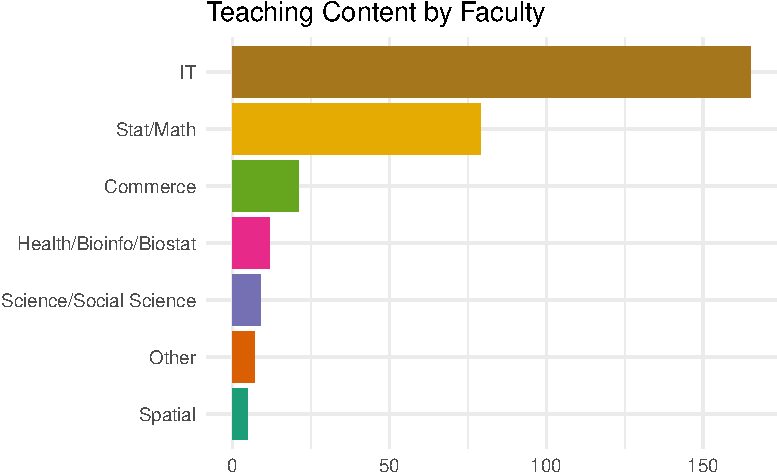
\includegraphics{./04_1-unitext_files/figure-pdf/fig-unitcode-1.pdf}

}

\caption{\label{fig-unitcode}Teaching Content by Faculty}

\end{figure}

Similar findings could be observed from some but not all Go8
universities. Figure~\ref{fig-unitcode-breakdown} shows the faculty
breakdown by university. Since the total number of units offered by each
university is different, instead of showing the actual number,
proportions are plotted to make better comparisons across universities.

\begin{figure}

{\centering 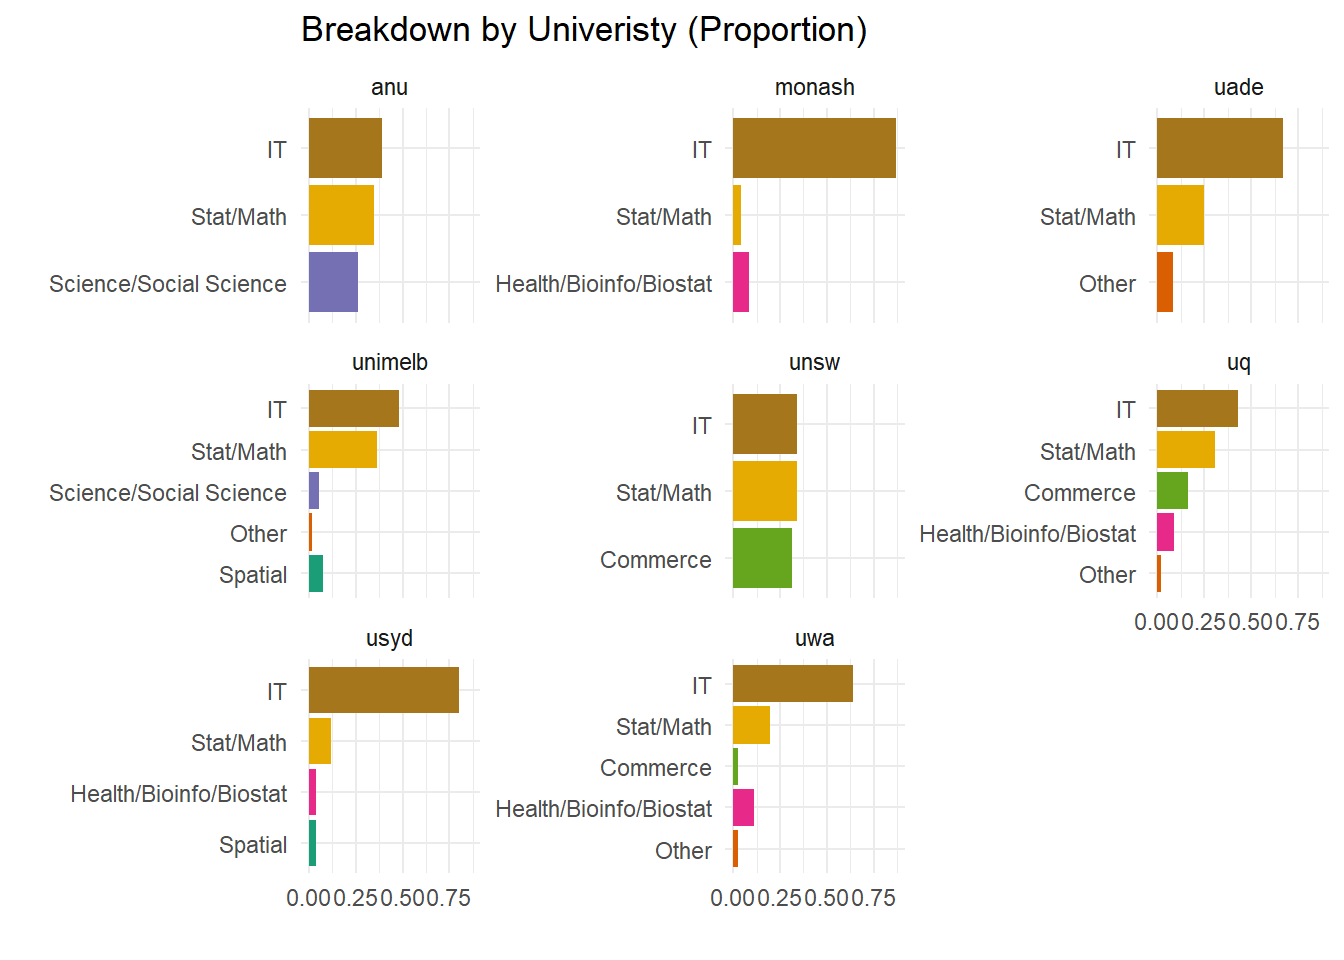
\includegraphics{./04_1-unitext_files/figure-pdf/fig-unitcode-breakdown-1.pdf}

}

\caption{\label{fig-unitcode-breakdown}Faculty Breakdown by University
(Proportion)}

\end{figure}

At Monash University (monash), University of Adelaide (Uuade),
University of Sydney (usyd) and University of Western Australia (uwa),
IT is apparently dominating the Master of Data Science degree,
especially at Monash University. However, University of Melbourne
(unimelb) and University of Queensland (uq) offers relatively higher
proportion of statistical and mathematical (Stat/Math) units, whereas
units offered at the Australian National University (anu) and UNSW
Sydney (unsw) are more evenly distributed across IT, Stat/Math,
Science/Social Science and Commerce respectively.

Based on the findings above, it seems that there is a shared structure
across Go8 that Master of Data Science is a IT based, computational
degree, but the proportion it occupies varies by universities. Monash
University tends to be heavily focused on IT and computational aspects,
whereas the Master of Data Science degree at UNSW Sydney and ANU are
more balanced across IT, statistics and math, as well as science and
commerce.

\hypertarget{sec-unit-bigram}{%
\section{Unit Overview and Learning Outcome -
Bigram}\label{sec-unit-bigram}}

After having a rough idea of the bigger picture, we then moved to
explore what exactly are the teaching contents. Single word analysis,
bigram and trigram are all produced in order to identify the frequently
mentioned words and/or terms. \texttt{distinct} function is applied to
unit and term, so that same terms are only counted once in a unit to
avoid duplicated counting. Words and terms such as `student',
`successful completion' add more noises than values to the results, are
removed in the pre-processing step.

The bigram, which is Figure~\ref{fig-bigram} below provides the most
informative results among all. Machine learning appears quite often, as
well as software development, linear models, statistical analysis,
spatial data. It seems that these frequently mentioned terms are
associated with both computational and statistical concepts and skills,
which aligns with the findings from the unit code analysis in previous
section.

\begin{figure}

{\centering 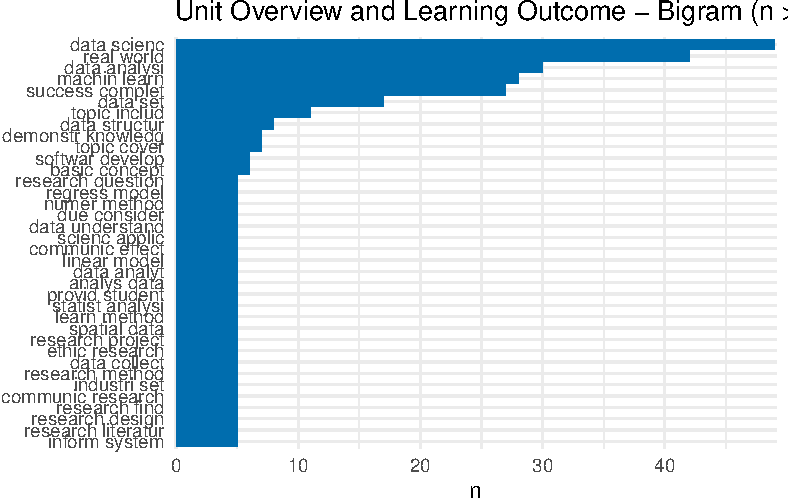
\includegraphics{./04_1-unitext_files/figure-pdf/fig-bigram-1.pdf}

}

\caption{\label{fig-bigram}Unit Overview and Learning Outcome - Bigram
(n \textgreater{} 4)}

\end{figure}

Unfortunately, due to the limited number of observations in the
collected data set, the count for each term is too low to make
meaningful interpretations or justifications. In addition, similar terms
such as research findings, research designs and research literature are
supposed to be grouped and counted together, but are not in the bigram.
This issue is later solved by introducing the text2vec technique for
natural language processing, which will be discussed in the next
chapter.

\hypertarget{job-text-analysis}{%
\chapter{Job Text Analysis}\label{job-text-analysis}}

To explore the skills and programming languages in demand from
employers, we focused on the mobileAdTemplate and the 25 columns of
programming languages. Similar to before, single word analysis, bigram,
and trigram are all produced.

\hypertarget{sec-word-frequency}{%
\section{Word Frequency}\label{sec-word-frequency}}

\begin{figure}

{\centering 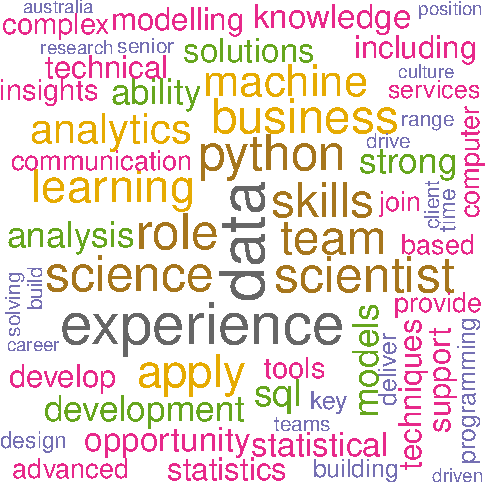
\includegraphics{./04_2-jobtext_files/figure-pdf/fig-job-freqency-1.pdf}

}

\caption{\label{fig-job-freqency}Job Word Frequency (freq
\textgreater200)}

\end{figure}

Word frequency was calculated using the same method as
Section~\ref{sec-unit-bigram}. Programming languages Python and SQL
seems prominent. Potentially due to the amount of senior positions in
the data, \emph{experience} is mentioned a lot. In terms of other
knowledge or skills, \emph{statistics}, \emph{modelling},
\emph{analysis} are some terms that seems to be standing out. To ensure
frequency is meaningful, we looked at bigram and trigram.

\hypertarget{bigram}{%
\section{Bigram}\label{bigram}}

\begin{figure}

{\centering 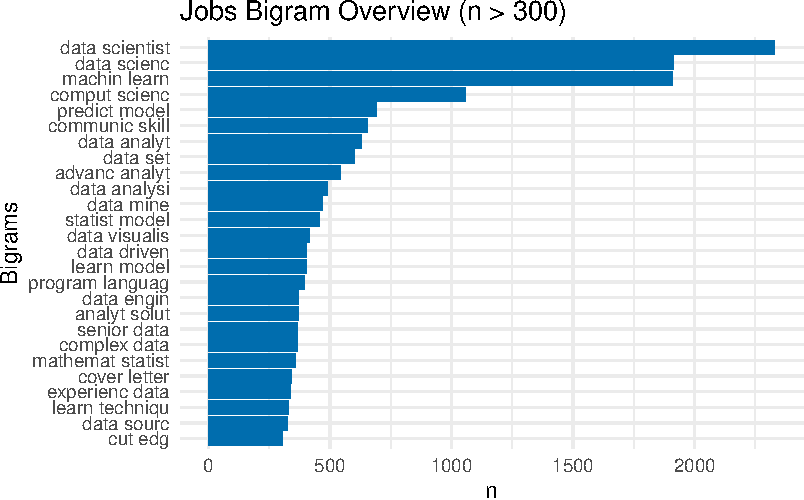
\includegraphics{./04_2-jobtext_files/figure-pdf/fig-employer-bigram-1.pdf}

}

\caption{\label{fig-employer-bigram}Job Description - Bigram (n
\textgreater{} 300}

\end{figure}

For Figure~\ref{fig-employer-bigram}, we stemmed the words before
joining them into bigram in attempt to avoid under-counting. However,
from the figure we can still see that some terms like \emph{data analyt}
and \emph{data analysi} are still counted separately. From this bigram,
the popular skills or knowledge mentioned are \emph{machin learn},
\emph{predict model}, \emph{communic skill}, \emph{data analyt} and
\emph{data mine}. Mathematical skill, \emph{mathemat statist} is also
mentioned quite often. Some of these terms on the list are vague and can
mean be grouped together. Trigram yeilded similar results as the bigram.
With the same problem of under-counting the n-grams due to insufficient
groupings.

\hypertarget{programming-languages}{%
\section{Programming Languages}\label{programming-languages}}

\begin{figure}

{\centering 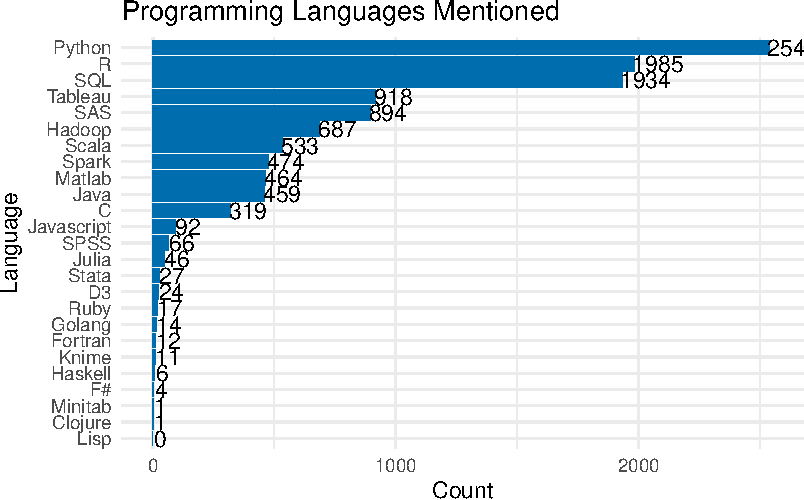
\includegraphics{./04_2-jobtext_files/figure-pdf/fig-languages-1.pdf}

}

\caption{\label{fig-languages}Programming Skills Mentioned by Employers}

\end{figure}

Figure~\ref{fig-languages} shows the count of each language mentioned by
employers. 89\% of the jobs mentioned Python, 69\% mentioned R and 68\%
mentioned SQL. Tableau's popularity is not a surprise given the high
frequency for \emph{data visualis} in the previous section.

\part{text2vec}

As mentioned in Section Section~\ref{sec-unit-bigram}, since the
collected university data is relatively small, to make more educated and
meaningful interpretations, similar words shall be grouped together and
counted by groups. This is usually computed using text corpus, which is
a language resource consisting of a large and structured set of texts,
since data science is a new term waiting to be defined, there is no
available text corpus on this topic. Therefore, we adopted the concept
of word2vec and tried to build our own text corpus.

There are multiple publicly available models and packages to conduct
similar computations, however, each model takes hours to fit. Due to
time constrains, we have only fitted the Dirichlet Allocation (LDA)
model with a few parameter adjustments using the \texttt{text2vec}
package with the concepts illustrated by Das (2016).

\hypertarget{algorithm-and-model-fitting}{%
\section*{Algorithm and Model
Fitting}\label{algorithm-and-model-fitting}}
\addcontentsline{toc}{section}{Algorithm and Model Fitting}

According to Das (2016), the algorithm behind the LDA model is to
convert words to document-term matrix (DTM), where the rows, columns and
entries correspond to documents, terms and counts respectively. LDA then
fits a probabilistic model that assumes a mixture of latent topics,
where each topic has a multinomial distribution for all words. The
number of topics is a parameter that could be adjusted by needs.

The initial code to build the LDA model was provided by Professor
Tanaka, the major part of the code to build the first version of LDA
model is also provided below.

\begin{Shaded}
\begin{Highlighting}[]
\FunctionTok{list}\NormalTok{(}
  \FunctionTok{tar\_target}\NormalTok{(wiki\_stats, }\FunctionTok{get\_wiki\_articles}\NormalTok{(}\StringTok{"https://en.wikipedia.org/wiki/List\_of\_statistics\_articles"}\NormalTok{)),}
  \FunctionTok{tar\_target}\NormalTok{(wiki\_sociology, }\FunctionTok{get\_wiki\_articles}\NormalTok{(}\StringTok{"https://en.wikipedia.org/wiki/Index\_of\_sociology\_articles"}\NormalTok{)),}
  \FunctionTok{tar\_target}\NormalTok{(wiki\_computing, }\FunctionTok{get\_wiki\_articles}\NormalTok{(}\StringTok{"https://en.wikipedia.org/wiki/Index\_of\_computing\_articles"}\NormalTok{)),}
  \FunctionTok{tar\_target}\NormalTok{(clean\_wiki\_stats, }\FunctionTok{map}\NormalTok{(wiki\_stats, clean\_wiki\_article), }\AttributeTok{format =} \StringTok{"rds"}\NormalTok{, }\AttributeTok{repository =} \StringTok{"local"}\NormalTok{),}
  \FunctionTok{tar\_target}\NormalTok{(clean\_wiki\_sociology, }\FunctionTok{map}\NormalTok{(wiki\_sociology, clean\_wiki\_article), }\AttributeTok{format =} \StringTok{"rds"}\NormalTok{, }\AttributeTok{repository =} \StringTok{"local"}\NormalTok{),}
  \FunctionTok{tar\_target}\NormalTok{(clean\_wiki\_computing, }\FunctionTok{map}\NormalTok{(wiki\_computing, clean\_wiki\_article), }\AttributeTok{format =} \StringTok{"rds"}\NormalTok{, }\AttributeTok{repository =} \StringTok{"local"}\NormalTok{),}
  \FunctionTok{tar\_target}\NormalTok{(clean\_stats, }\FunctionTok{preprocess\_text}\NormalTok{(clean\_wiki\_stats)),}
  
  \FunctionTok{tar\_target}\NormalTok{(clean\_ssc, }\FunctionTok{preprocess\_text}\NormalTok{(}\FunctionTok{c}\NormalTok{(clean\_wiki\_stats, clean\_wiki\_sociology, clean\_wiki\_computing))),}
  
  \FunctionTok{tar\_target}\NormalTok{(itoken\_ssc, }\FunctionTok{itoken}\NormalTok{(clean\_ssc, }\AttributeTok{tokenizer =}\NormalTok{ stem\_tokenizer),}
             \AttributeTok{cue =} \FunctionTok{tar\_cue}\NormalTok{(}\AttributeTok{mode =} \StringTok{"thorough"}\NormalTok{)),}
 
  \FunctionTok{tar\_target}\NormalTok{(vocab\_ssc, }\FunctionTok{create\_vocabulary}\NormalTok{(itoken\_ssc, }\AttributeTok{ngram =} \FunctionTok{c}\NormalTok{(}\DecValTok{1}\NormalTok{, }\DecValTok{3}\NormalTok{), }\AttributeTok{stopwords =}\NormalTok{ stopwords}\SpecialCharTok{::}\FunctionTok{stopwords}\NormalTok{()),}
             \AttributeTok{cue =} \FunctionTok{tar\_cue}\NormalTok{(}\AttributeTok{mode =} \StringTok{"thorough"}\NormalTok{)),}
  \FunctionTok{tar\_target}\NormalTok{(vocab\_ssc\_prune, }\FunctionTok{prune\_vocab}\NormalTok{(vocab\_ssc, }\AttributeTok{n\_min =} \DecValTok{40}\NormalTok{),}
             \AttributeTok{cue =} \FunctionTok{tar\_cue}\NormalTok{(}\AttributeTok{mode =} \StringTok{"thorough"}\NormalTok{)),}
  \FunctionTok{tar\_target}\NormalTok{(dtm\_ssc, }\FunctionTok{create\_dtm}\NormalTok{(itoken\_ssc, }\FunctionTok{vocab\_vectorizer}\NormalTok{(vocab\_ssc\_prune)),}
             \AttributeTok{cue =} \FunctionTok{tar\_cue}\NormalTok{(}\AttributeTok{mode =} \StringTok{"thorough"}\NormalTok{)),}
  \FunctionTok{tar\_target}\NormalTok{(tcm\_ssc, }\FunctionTok{create\_tcm}\NormalTok{(itoken\_ssc, }\FunctionTok{vocab\_vectorizer}\NormalTok{(vocab\_ssc\_prune), }
                                 \AttributeTok{skip\_grams\_window =}\NormalTok{ 5L),}
             \AttributeTok{cue =} \FunctionTok{tar\_cue}\NormalTok{(}\AttributeTok{mode =} \StringTok{"thorough"}\NormalTok{)),}
  \FunctionTok{tar\_target}\NormalTok{(word2vec\_model\_ssc, }\FunctionTok{model\_glove}\NormalTok{(vocab\_ssc\_prune, tcm\_ssc),}
             \AttributeTok{cue =} \FunctionTok{tar\_cue}\NormalTok{(}\AttributeTok{mode =} \StringTok{"thorough"}\NormalTok{)),}
  \FunctionTok{tar\_target}\NormalTok{(word2vec\_dist\_ssc, }\FunctionTok{dist2}\NormalTok{(}\FunctionTok{t}\NormalTok{(word2vec\_model\_ssc}\SpecialCharTok{$}\NormalTok{components), }\AttributeTok{method =} \StringTok{"cosine"}\NormalTok{),}
             \AttributeTok{cue =} \FunctionTok{tar\_cue}\NormalTok{(}\AttributeTok{mode =} \StringTok{"thorough"}\NormalTok{), }\AttributeTok{format =} \StringTok{"rds"}\NormalTok{, }\AttributeTok{repository =} \StringTok{"local"}\NormalTok{),}
  \FunctionTok{tar\_target}\NormalTok{(word2vec\_res, }\FunctionTok{find\_close\_words}\NormalTok{(}\StringTok{"statistics"}\NormalTok{, word2vec\_dist\_ssc, }\DecValTok{10}\NormalTok{),}
             \AttributeTok{cue =} \FunctionTok{tar\_cue}\NormalTok{(}\AttributeTok{mode =} \StringTok{"thorough"}\NormalTok{)),}
  \FunctionTok{tar\_target}\NormalTok{(lda\_model03\_ssc, }\FunctionTok{model\_lda}\NormalTok{(dtm\_ssc, }\AttributeTok{ntopics =} \DecValTok{3}\NormalTok{),}
             \AttributeTok{format =} \StringTok{"rds"}\NormalTok{, }\AttributeTok{repository =} \StringTok{"local"}\NormalTok{),}
  \FunctionTok{tar\_target}\NormalTok{(lda\_model20\_ssc, }\FunctionTok{model\_lda}\NormalTok{(dtm\_ssc, }\AttributeTok{ntopics =} \DecValTok{20}\NormalTok{),}
             \AttributeTok{format =} \StringTok{"rds"}\NormalTok{, }\AttributeTok{repository =} \StringTok{"local"}\NormalTok{)}
\NormalTok{             )}
\end{Highlighting}
\end{Shaded}

The model must be trained before it could be used, we web scraped over
4448 Wikipedia articles as training data, including 2816 articles in
statistics, 1005 articles in sociology and 627 in computing. The
functions used in the codes above such as
\texttt{get\_wiki\_articles},\texttt{clean\_wiki\_article},
\texttt{get\_clean\_combined\_wikis}, \texttt{model\_lda},
\texttt{preprocess\_text}, \texttt{stem\_tokenizer},
\texttt{prune\_vocab}, \texttt{model\_glove} and
\texttt{find\_close\_words} are constructed by Professor Tanaka for
pre-processing purposes, the original scripts could be found from the
\href{https://github.com/numbats/datasci-courses}{project repository}.

\hypertarget{model-adjustments}{%
\section*{Model Adjustments}\label{model-adjustments}}
\addcontentsline{toc}{section}{Model Adjustments}

We have tested using different values for parameter \texttt{ntopics} and
tried out training the LDA models with different combinations of data.

The results provided differs from models, Figure~\ref{fig-ssc-cs}
compares the results produced by the full model and model without
sociology data on ten topics.

\begin{figure}

{\centering 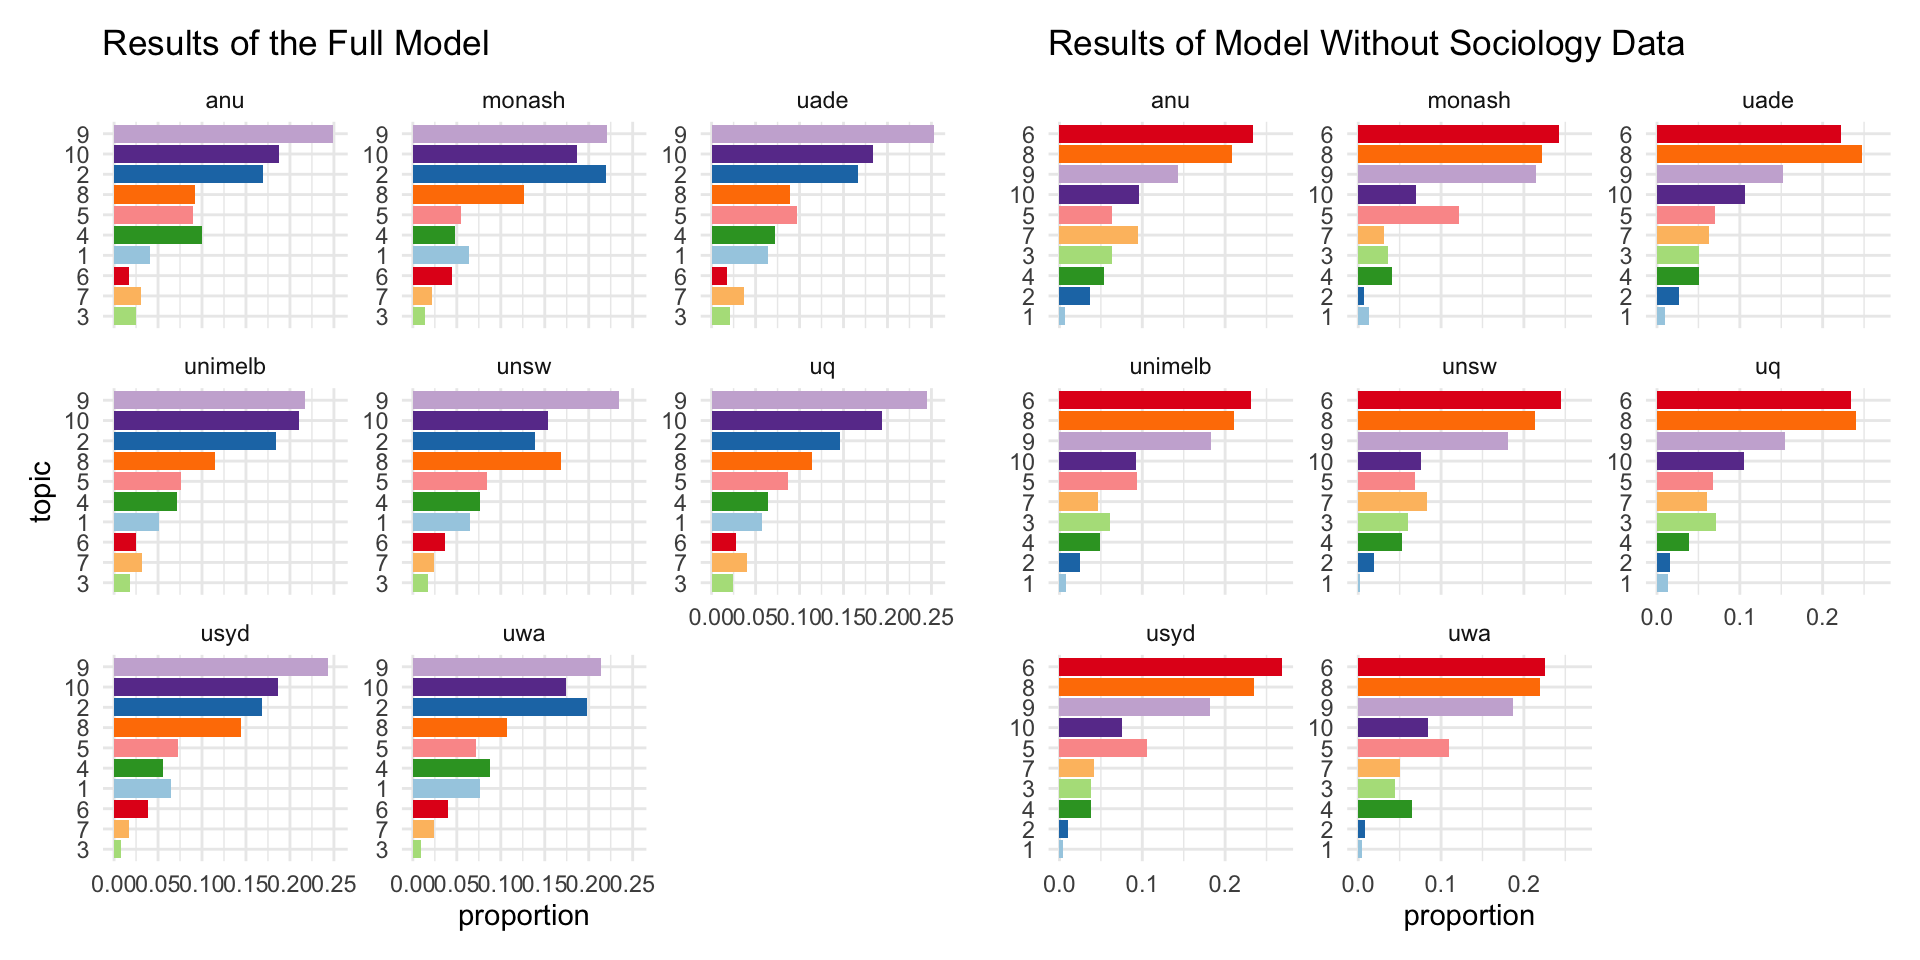
\includegraphics{./05-text2vec_files/figure-pdf/fig-ssc-cs-1.pdf}

}

\caption{\label{fig-ssc-cs}Compare Results Between Full Model and
Without Sociology Data}

\end{figure}

From the results computed by the full model, Topics 9, 10, 2 and 8
occupies relatively higher proportion compare with the others, but the
order varies across universities, and their proportions are not
significantly larger than the rest of other topics, makes it hard to
draw meaningful interpretations. On the right hand side, results from
the model without sociology data demonstrates a better picture: Topics
6, 8 and 9 in this case are the top 3 topics across all Go8
universities, however, proportions of Topic 10, 5, 7, 3 and 4 are also
obvious higher in some of the universities, brings in difficulties to
make justifications.

As sociology data tends to brings in noises to the model, and is not
closely relevant to the data science topic compare with statistics and
computing, another two models are fitted using only statistics data and
computing data respectively, the results of both models are shown in
Figure~\ref{fig-comp-stats}.

\begin{figure}

{\centering 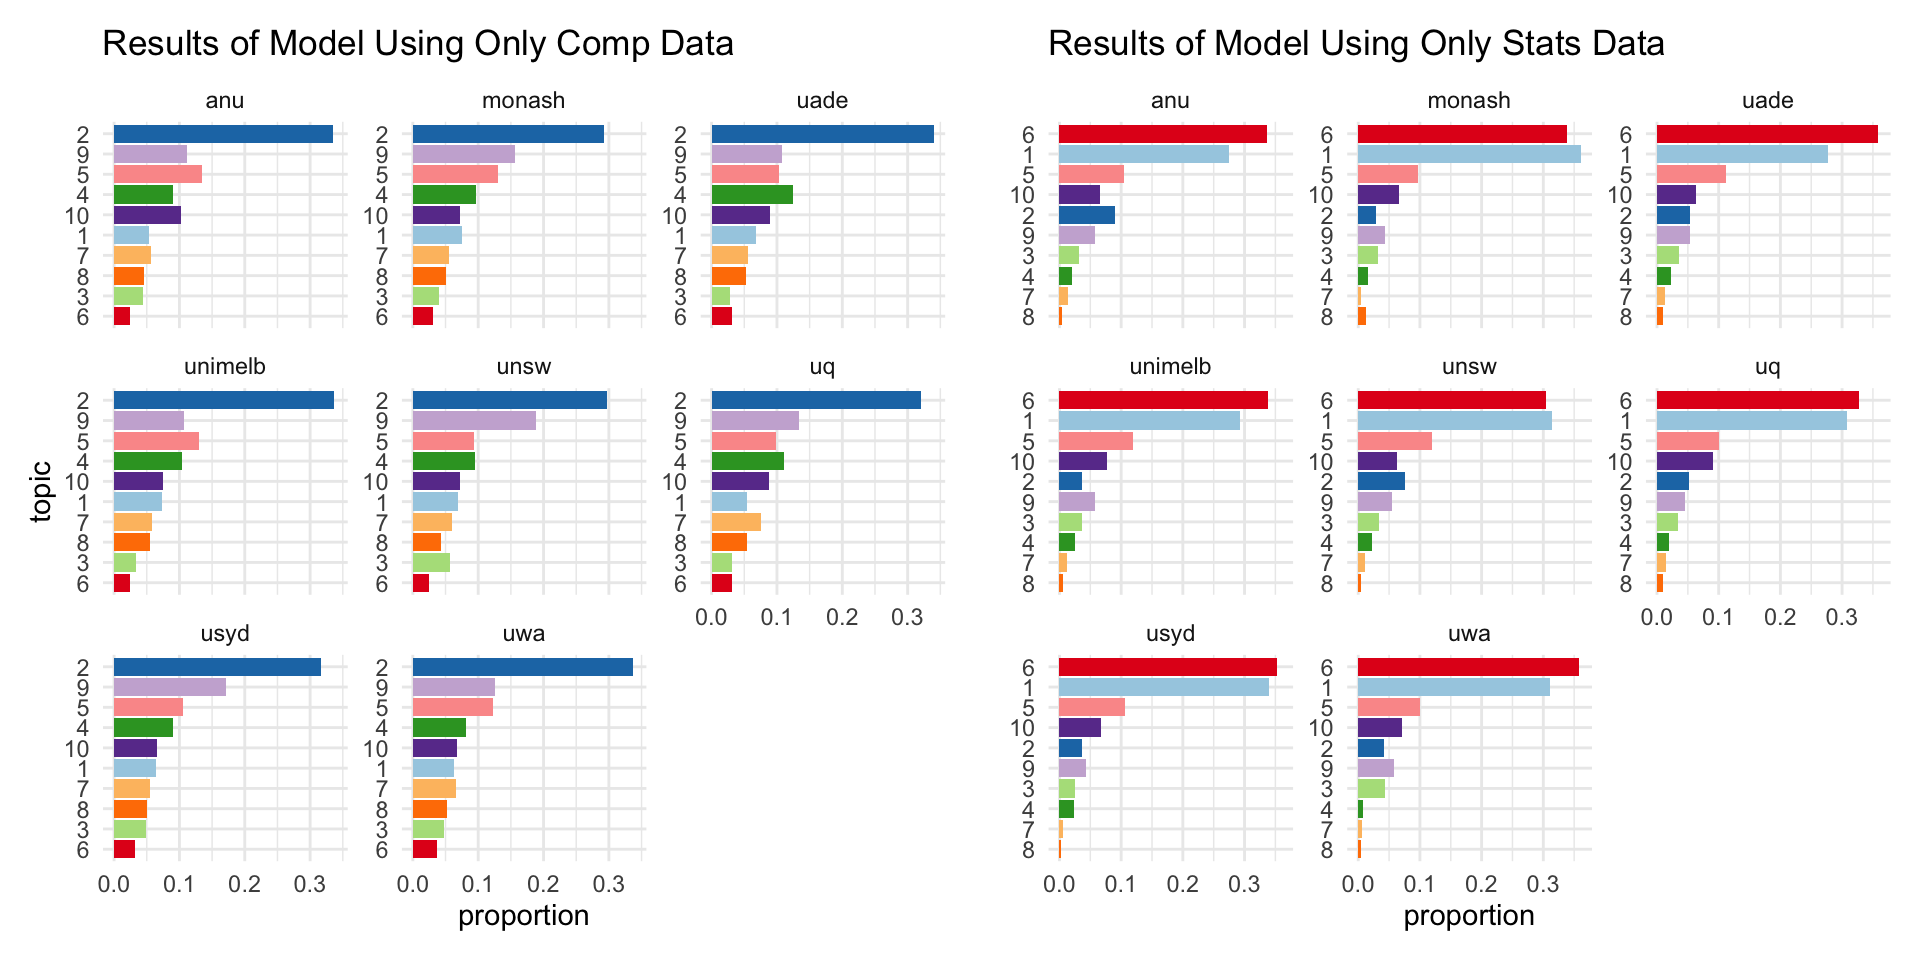
\includegraphics{./05-text2vec_files/figure-pdf/fig-comp-stats-1.pdf}

}

\caption{\label{fig-comp-stats}Compare Results Between Full Model and
Without Sociology Data}

\end{figure}

Topic 2 is the only dominating topic based on the results provided by
the model using only computing data, which provides a clearer picture
than the previous models. The table below listed the top ten words for
each topics, it turns out Topic 2 contains words like comput
(computation etc.), system, program, softwar (software), which are
associated with computational aspects, especially software. This model
provides a more meaningful results than the prior ones, however, there
is not much interpretations could be made for the other topics, the
information it offers is still not very satisfying.

\begin{table}
\centering
\begin{tabular}{l|l|l|l|l|l|l|l|l|l}
\hline
Topic 1 & Topic 2 & Topic 3 & Topic 4 & Topic 5 & Topic 6 & Topic 7 & Topic 8 & Topic 9 & Topic 10\\
\hline
window & comput & ibm & algorithm & network & bit & format & intel & softwar & languag\\
\hline
system & system & comput & can & use & instruct & use & chip & compani & program\\
\hline
version & program & system & number & can & memori & imag & design & appl & use\\
\hline
releas & use & disk & function & web & use & digit & processor & free & compil\\
\hline
support & machin & drive & set & data & address & can & bit & use & code\\
\hline
user & design & use & state & internet & regist & video & core & also & function\\
\hline
oper\_system & process & control & languag & secur & processor & standard & mhz & develop & object\\
\hline
oper & develop & machin & use & access & oper & disc & use & open & type\\
\hline
os & inform & card & symbol & protocol & can & data & introduc & sourc & can\\
\hline
file & softwar & unit & problem & link & data & file & microprocessor & user & implement\\
\hline
\end{tabular}
\end{table}

In terms of the model trained by only data in statistics, there are also
dominating topics across all eight universities: Topics 6 and 1,
besides, topics 5, 10, 2, 9 together took a relatively higher proportion
compare with the rest of other topics. Both models using only computing
or statistical data delivers better results, model trained by only
statistical data provides more information than the other, hence is
selected to use for further analysis on our university data.

Note that it requires highly skilled linguists and huge efforts to
establish a proper text corpus, the model we built is still fairly basic
and could be further optimised by adjustments.

\hypertarget{apply-the-selected-model-to-collected-university-data}{%
\chapter{Apply the Selected Model to Collected University
Data}\label{apply-the-selected-model-to-collected-university-data}}

Before applying the fitted LDA model to our university data set, words
from unit overview and learning outcomes are stemmed using the
\texttt{SnowballC} package, so that noises like plurals and part of
speech are removed. The stemmed words are then assigned to the
corresponding topic with the highest probability, instead of counting
the appearance of words, the new counts generated are based on topics.

Similar with the university breakdown in Section~\ref{sec-unit-bigram},
to make more objective comparisons, counts are converted to proportions
due to different number of units scraped for the eight universities.
Figure~\ref{fig-unitopics} suggests that Topics 1 and 6 are obviously
the dominating topics in Master of data science at all Go8 universities,
whereas Topics 2, 5, 9, 10 together also occupies a relatively large
proportion.

\begin{figure}

{\centering 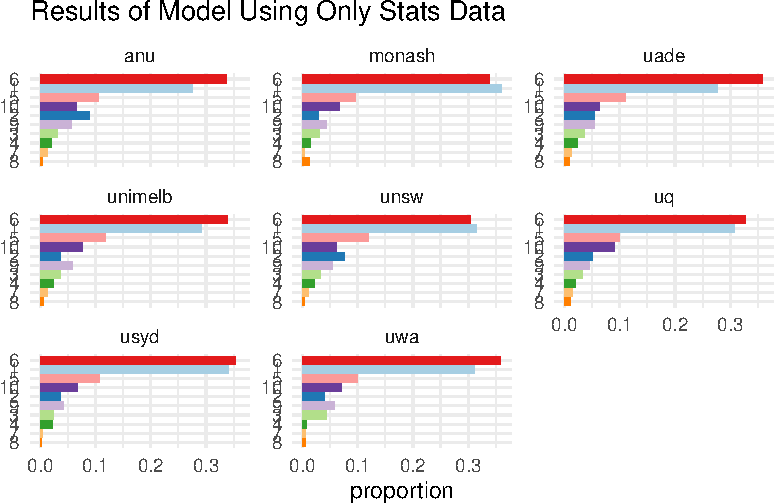
\includegraphics{./05_1-unilda_files/figure-pdf/fig-unitopics-1.pdf}

}

\caption{\label{fig-unitopics}Topics Proportion by University}

\end{figure}

The top ten words based on probabilities for each of the ten topics are
provided below, colours of the columns are aligned with
Figure~\ref{fig-unitopics}. Topic 1 contains words like statist
(statistics), data, popul (population), and we can see data, algorithm,
analysi (analysis), model, cluster, comput (computation etc.) in topic
6, it is a reasonable interpretation that these two topics are both
associated with computational aspects.

\begin{figure}

{\centering 

\hypertarget{fig-topics-1}{}
\begin{table}
\centering\begingroup\fontsize{12}{14}\selectfont

\begin{tabular}{>{}l|>{}l|>{}l|>{}l|>{}l|>{}l|>{}l|>{}l|>{}l|>{}l}
\hline
Topic 1 & Topic 2 & Topic 3 & Topic 4 & Topic 5 & Topic 6 & Topic 7 & Topic 8 & Topic 9 & Topic 10\\
\hline
\cellcolor[HTML]{A6CEE3}{\textcolor{white}{studi}} & \cellcolor[HTML]{1F78B4}{\textcolor{white}{model}} & \cellcolor[HTML]{B2DF8A}{\textcolor{white}{sampl}} & \cellcolor[HTML]{33A02C}{\textcolor{white}{theta}} & \cellcolor[HTML]{FB9A99}{\textcolor{white}{probabl}} & \cellcolor[HTML]{E31A1C}{\textcolor{white}{data}} & \cellcolor[HTML]{FDBF6F}{\textcolor{white}{distribut}} & \cellcolor[HTML]{FF7F00}{\textcolor{white}{x\_}} & \cellcolor[HTML]{CAB2D6}{\textcolor{white}{test}} & \cellcolor[HTML]{6A3D9A}{\textcolor{white}{process}}\\
\hline
\cellcolor[HTML]{A6CEE3}{\textcolor{white}{use}} & \cellcolor[HTML]{1F78B4}{\textcolor{white}{variabl}} & \cellcolor[HTML]{B2DF8A}{\textcolor{white}{estim}} & \cellcolor[HTML]{33A02C}{\textcolor{white}{function}} & \cellcolor[HTML]{FB9A99}{\textcolor{white}{one}} & \cellcolor[HTML]{E31A1C}{\textcolor{white}{use}} & \cellcolor[HTML]{FDBF6F}{\textcolor{white}{frac}} & \cellcolor[HTML]{FF7F00}{\textcolor{white}{frac}} & \cellcolor[HTML]{CAB2D6}{\textcolor{white}{statist}} & \cellcolor[HTML]{6A3D9A}{\textcolor{white}{time}}\\
\hline
\cellcolor[HTML]{A6CEE3}{\textcolor{white}{statist}} & \cellcolor[HTML]{1F78B4}{\textcolor{white}{regress}} & \cellcolor[HTML]{B2DF8A}{\textcolor{white}{mean}} & \cellcolor[HTML]{33A02C}{\textcolor{white}{probabl}} & \cellcolor[HTML]{FB9A99}{\textcolor{white}{number}} & \cellcolor[HTML]{E31A1C}{\textcolor{white}{algorithm}} & \cellcolor[HTML]{FDBF6F}{\textcolor{white}{alpha}} & \cellcolor[HTML]{FF7F00}{\textcolor{white}{left}} & \cellcolor[HTML]{CAB2D6}{\textcolor{white}{hypothesi}} & \cellcolor[HTML]{6A3D9A}{\textcolor{white}{point}}\\
\hline
\cellcolor[HTML]{A6CEE3}{\textcolor{white}{research}} & \cellcolor[HTML]{1F78B4}{\textcolor{white}{estim}} & \cellcolor[HTML]{B2DF8A}{\textcolor{white}{valu}} & \cellcolor[HTML]{33A02C}{\textcolor{white}{x\_x}} & \cellcolor[HTML]{FB9A99}{\textcolor{white}{theori}} & \cellcolor[HTML]{E31A1C}{\textcolor{white}{analysi}} & \cellcolor[HTML]{FDBF6F}{\textcolor{white}{mu}} & \cellcolor[HTML]{FF7F00}{\textcolor{white}{right}} & \cellcolor[HTML]{CAB2D6}{\textcolor{white}{valu}} & \cellcolor[HTML]{6A3D9A}{\textcolor{white}{stochast}}\\
\hline
\cellcolor[HTML]{A6CEE3}{\textcolor{white}{data}} & \cellcolor[HTML]{1F78B4}{\textcolor{white}{beta}} & \cellcolor[HTML]{B2DF8A}{\textcolor{white}{distribut}} & \cellcolor[HTML]{33A02C}{\textcolor{white}{distribut}} & \cellcolor[HTML]{FB9A99}{\textcolor{white}{bayesian}} & \cellcolor[HTML]{E31A1C}{\textcolor{white}{can}} & \cellcolor[HTML]{FDBF6F}{\textcolor{white}{beta}} & \cellcolor[HTML]{FF7F00}{\textcolor{white}{sum}} & \cellcolor[HTML]{CAB2D6}{\textcolor{white}{two}} & \cellcolor[HTML]{6A3D9A}{\textcolor{white}{state}}\\
\hline
\cellcolor[HTML]{A6CEE3}{\textcolor{white}{design}} & \cellcolor[HTML]{1F78B4}{\textcolor{white}{linear}} & \cellcolor[HTML]{B2DF8A}{\textcolor{white}{varianc}} & \cellcolor[HTML]{33A02C}{\textcolor{white}{variabl}} & \cellcolor[HTML]{FB9A99}{\textcolor{white}{event}} & \cellcolor[HTML]{E31A1C}{\textcolor{white}{method}} & \cellcolor[HTML]{FDBF6F}{\textcolor{white}{function}} & \cellcolor[HTML]{FF7F00}{\textcolor{white}{operatornam}} & \cellcolor[HTML]{CAB2D6}{\textcolor{white}{number}} & \cellcolor[HTML]{6A3D9A}{\textcolor{white}{function}}\\
\hline
\cellcolor[HTML]{A6CEE3}{\textcolor{white}{can}} & \cellcolor[HTML]{1F78B4}{\textcolor{white}{use}} & \cellcolor[HTML]{B2DF8A}{\textcolor{white}{statist}} & \cellcolor[HTML]{33A02C}{\textcolor{white}{random}} & \cellcolor[HTML]{FB9A99}{\textcolor{white}{can}} & \cellcolor[HTML]{E31A1C}{\textcolor{white}{model}} & \cellcolor[HTML]{FDBF6F}{\textcolor{white}{gamma}} & \cellcolor[HTML]{FF7F00}{\textcolor{white}{sigma}} & \cellcolor[HTML]{CAB2D6}{\textcolor{white}{use}} & \cellcolor[HTML]{6A3D9A}{\textcolor{white}{can}}\\
\hline
\cellcolor[HTML]{A6CEE3}{\textcolor{white}{effect}} & \cellcolor[HTML]{1F78B4}{\textcolor{white}{y\_}} & \cellcolor[HTML]{B2DF8A}{\textcolor{white}{use}} & \cellcolor[HTML]{33A02C}{\textcolor{white}{x\_}} & \cellcolor[HTML]{FB9A99}{\textcolor{white}{prior}} & \cellcolor[HTML]{E31A1C}{\textcolor{white}{set}} & \cellcolor[HTML]{FDBF6F}{\textcolor{white}{right}} & \cellcolor[HTML]{FF7F00}{\textcolor{white}{y\_}} & \cellcolor[HTML]{CAB2D6}{\textcolor{white}{correl}} & \cellcolor[HTML]{6A3D9A}{\textcolor{white}{random}}\\
\hline
\cellcolor[HTML]{A6CEE3}{\textcolor{white}{popul}} & \cellcolor[HTML]{1F78B4}{\textcolor{white}{squar}} & \cellcolor[HTML]{B2DF8A}{\textcolor{white}{standard}} & \cellcolor[HTML]{33A02C}{\textcolor{white}{random\_variabl}} & \cellcolor[HTML]{FB9A99}{\textcolor{white}{infer}} & \cellcolor[HTML]{E31A1C}{\textcolor{white}{cluster}} & \cellcolor[HTML]{FDBF6F}{\textcolor{white}{left}} & \cellcolor[HTML]{FF7F00}{\textcolor{white}{cdot}} & \cellcolor[HTML]{CAB2D6}{\textcolor{white}{rank}} & \cellcolor[HTML]{6A3D9A}{\textcolor{white}{markov}}\\
\hline
\cellcolor[HTML]{A6CEE3}{\textcolor{white}{may}} & \cellcolor[HTML]{1F78B4}{\textcolor{white}{can}} & \cellcolor[HTML]{B2DF8A}{\textcolor{white}{popul}} & \cellcolor[HTML]{33A02C}{\textcolor{white}{mathcal}} & \cellcolor[HTML]{FB9A99}{\textcolor{white}{use}} & \cellcolor[HTML]{E31A1C}{\textcolor{white}{comput}} & \cellcolor[HTML]{FDBF6F}{\textcolor{white}{normal}} & \cellcolor[HTML]{FF7F00}{\textcolor{white}{operatornam\_e}} & \cellcolor[HTML]{CAB2D6}{\textcolor{white}{measur}} & \cellcolor[HTML]{6A3D9A}{\textcolor{white}{space}}\\
\hline
\end{tabular}
\endgroup{}
\end{table}

}

\caption{\label{fig-topics}Top 10 words of the Ten Topics}

\end{figure}

In addition, words under Topics 2,5,9 and 10 are model, regression,
estim (estimate), linear, probabl (probability), bayesian, prior, infer,
test, statist (statistics), hypothesi (hypothesis), correl
(correlation), most of them are related to math and statistics, and also
more on the computational side of them.

The results above further proves the earlier findings discussed in
Section~\ref{sec-unit-code} and Section~\ref{sec-unit-bigram}: Master of
Data Science degrees offered at Go8 universities tend to be mainly IT
based, the major components are computational as well as
statistical/mathematical aspects.

\begin{figure}

{\centering 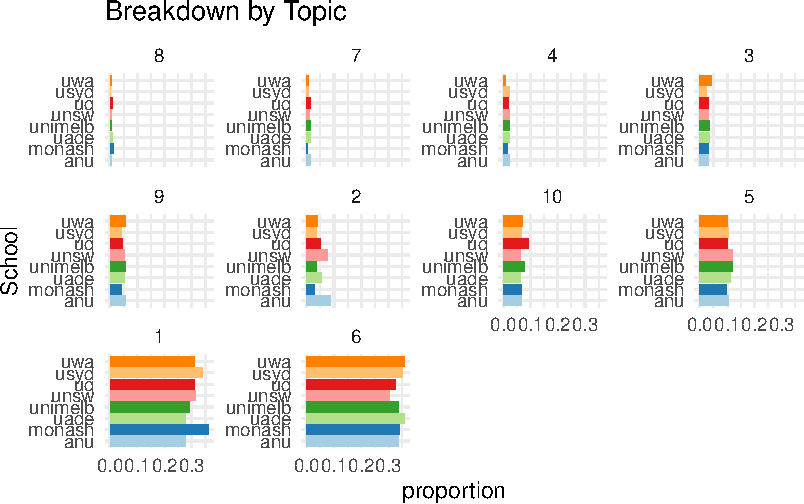
\includegraphics{./05_1-unilda_files/figure-pdf/fig-unitopics2-1.pdf}

}

\caption{\label{fig-unitopics2}Proportion Breakdown by Topic}

\end{figure}

Figure~\ref{fig-unitopics2} demonstrates a breakdown by topics instead
of universities, it is clear that compares with the results based on
only faculty in Section~\ref{sec-unit-code}, the differences between Go8
are not as much here. The proportions occupied by the eight universities
under each topic are fairly similar to each other, indicating the
subjective choice made regarding the grouping method in
Section~\ref{sec-unit-code} might have provided a slightly misleading
information, but it would require further explorations to confirm
whether it is truly the case.

\hypertarget{apply-the-selected-model-to-employer-data}{%
\chapter{Apply the Selected Model to Employer
Data}\label{apply-the-selected-model-to-employer-data}}

To remain consistent with the analysis, we also applied the LDA model
trained by only data in statistics to the employer data with the same
stemming and standardizing procedures. Unlike the university data with
both Topic 6 and 1 as the most dominant topics, Figure~\ref{fig-emp-lda}
suggests that Topic 1 is significantly more dominant than the rest of
the topics across the different job sectors. While Topic 6 and 5
collectively takes up a large portion.

\begin{figure}

{\centering 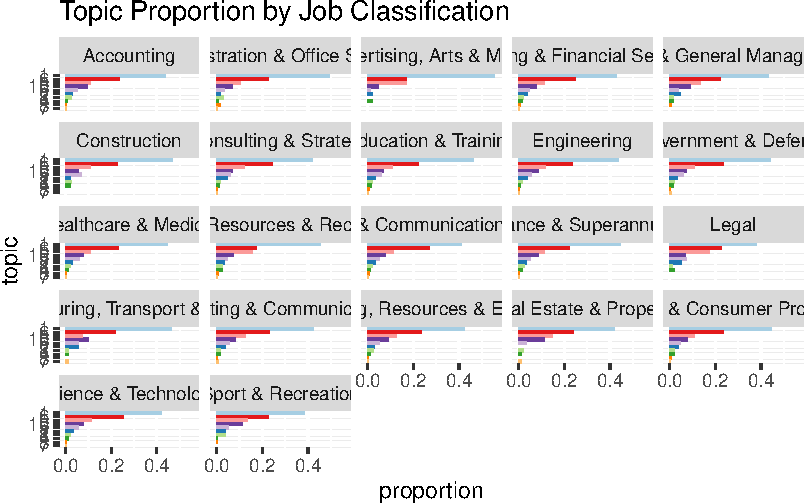
\includegraphics{./05_2-joblda_files/figure-pdf/fig-emp-lda-1.pdf}

}

\caption{\label{fig-emp-lda}Topics Proportion by Job Classification}

\end{figure}

Since the same LDA model is being applied, the breakdown of words in
each topic can be found in Figure~\ref{fig-topics}. Topic 1 has data and
statist in its top 10 words, which are also popular words found in
Figure~\ref{fig-job-freqency}. Topics 1, 6, 5 are all computational and
some statistical elements. Hence we can conclude that both the employers
universities have a more computational approach to data science.
However, the magnitude of effect for the difference in proportion of
topics is not being measured here.

\bookmarksetup{startatroot}

\hypertarget{conclusion}{%
\chapter{Conclusion}\label{conclusion}}

\hypertarget{summary}{%
\section{Summary}\label{summary}}

\hypertarget{limitation}{%
\section{Limitation}\label{limitation}}

\hypertarget{furture-directions}{%
\section{Furture Directions}\label{furture-directions}}

\bookmarksetup{startatroot}

\hypertarget{references}{%
\chapter*{References}\label{references}}
\addcontentsline{toc}{chapter}{References}

\hypertarget{refs}{}
\begin{CSLReferences}{1}{0}
\leavevmode\vadjust pre{\hypertarget{ref-das2016data}{}}%
Das, Sanjiv Ranjan. 2016. {``Data Science: Theories, Models, Algorithms,
and Analytics.''} \emph{Learning} 143: 145.

\end{CSLReferences}



\end{document}
